% !TeX document-id = {248a0dfa-b565-486e-ba41-17b905998a24}
% !TeX TS-program = pdflatex
% !BIB TS-program = biber
% !TeX root = main.tex
\documentclass[
normalmargins,
12pt,
openany,
onehalfspacing,
]{ut-thesis}

% Adjust the margin's length and line spacing
\usepackage{geometry}
\usepackage{setspace}
\geometry{left=1.5in,right=1.0in,top=1.0in,bottom=1.0in,includefoot}
\doublespacing

% Initally use roman numbering
\pagenumbering{roman}

% Adjust the appearance of the Table of Contents
\usepackage{tocbibind}
\usepackage[titles]{tocloft}

% packages
\usepackage[utf8]{inputenc}

\usepackage[colorlinks]{hyperref} % for links
\usepackage[backend=biber]{biblatex} % for references
\usepackage{graphicx} % for embedding graphics
\usepackage{booktabs} % for pretty tables
\usepackage{amsmath}
\usepackage{amsthm}
\usepackage{algorithm2e}
\usepackage{amssymb}
\usepackage{latexsym}
\usepackage{lipsum} % for gibberish text
\usepackage{todonotes}
\usepackage{tabularx}
\usepackage{svg}
\usepackage{caption}
\usepackage{subcaption}
\usepackage{multirow}
\usepackage{fvextra}
\usepackage{bm}
\usepackage{pdfpages}

\setlength {\marginparwidth }{2cm}
\setcounter{secnumdepth}{5}
\svgpath{{my/graphics/}}

% list of abbreviations
\usepackage[intoc]{nomencl}
\makenomenclature
\renewcommand{\nomname}{List of Abbreviations}% and Symbols

\newtheorem{definition}{Definition}
\newtheorem{theorem}{Theorem}
\theoremstyle{definition} % switch to 'definition' theorem style
\newtheorem{example}{Example}

\newcommand\floorbrackets[1]{\ensuremath{%
		\bm{\lfloor}\mkern-1mu%
		\text{#1}%
		\bm{\rfloor}}}

\newcommand{\Attr}{\operatorname{attr}}
\newcommand{\Field}{\operatorname{field}}
\newcommand{\Values}{\mathbf{Values}}
\newcommand{\Token}{\mathbf{Token}}
\newcommand{\List}{\mathbf{List}}
\newcommand{\Sim}{\mathrm{sim}}
\newcommand{\Tokenize}{\mathbf{tokenize}}

\newcommand{\thesisTitle}[8]{
	\title{#2}
	\author{#1}

	\begin{titlepage}
		\centering
		\textbf{\large #2}
		\\[1cm]

		by
		\\[1cm]

		#1 % author
		\\[1.0cm]

		\begin{minipage}{4in}
			\centering
			\singlespacing{A thesis submitted to the \\ School of Graduate and Postdoctoral Studies in partial fulfillment of the requirements for the degree of}
		\end{minipage}
		\\[1.5cm]

		\textbf{#3} % degree name
		\\[1.5cm]

		#4 % faculty name
		\\[0.25cm]

		#5 % school name
		\\[0.25cm]

		#6 % address
		\\[0.25cm]

		#7 #8
		\\[0.5cm]

		{\copyright\ #1, #8}
	\end{titlepage}
}

\usepackage{hyperref}
\hypersetup{
	colorlinks,
	citecolor=black,
	filecolor=black,
	linkcolor=black,
	urlcolor=black
}

%\linespread{2}
%\author{Limin Ma}
\title{Optimizing Relational Search With Embedded Neural Network}
\degree{Master of Science in Computer Science}
\department{Faculty of Science}
\gradyear{2023}

% reference database

\addbibresource{my/references.bib}

\begin{document}
%\frontmatter

\thesisTitle
	{Limin Ma}
	{Optimizing Relational Search With Embedded Neural Network}
	{Master of Science in Computer Science}
	{Faculty of Science}
	{University of Ontario Institute of Technology (Ontario Tech University)}
	{Oshawa, Ontario, Canada}
	{April}
	{2023}

\phantomsection\addcontentsline{toc}{chapter}{Thesis Examination Information}
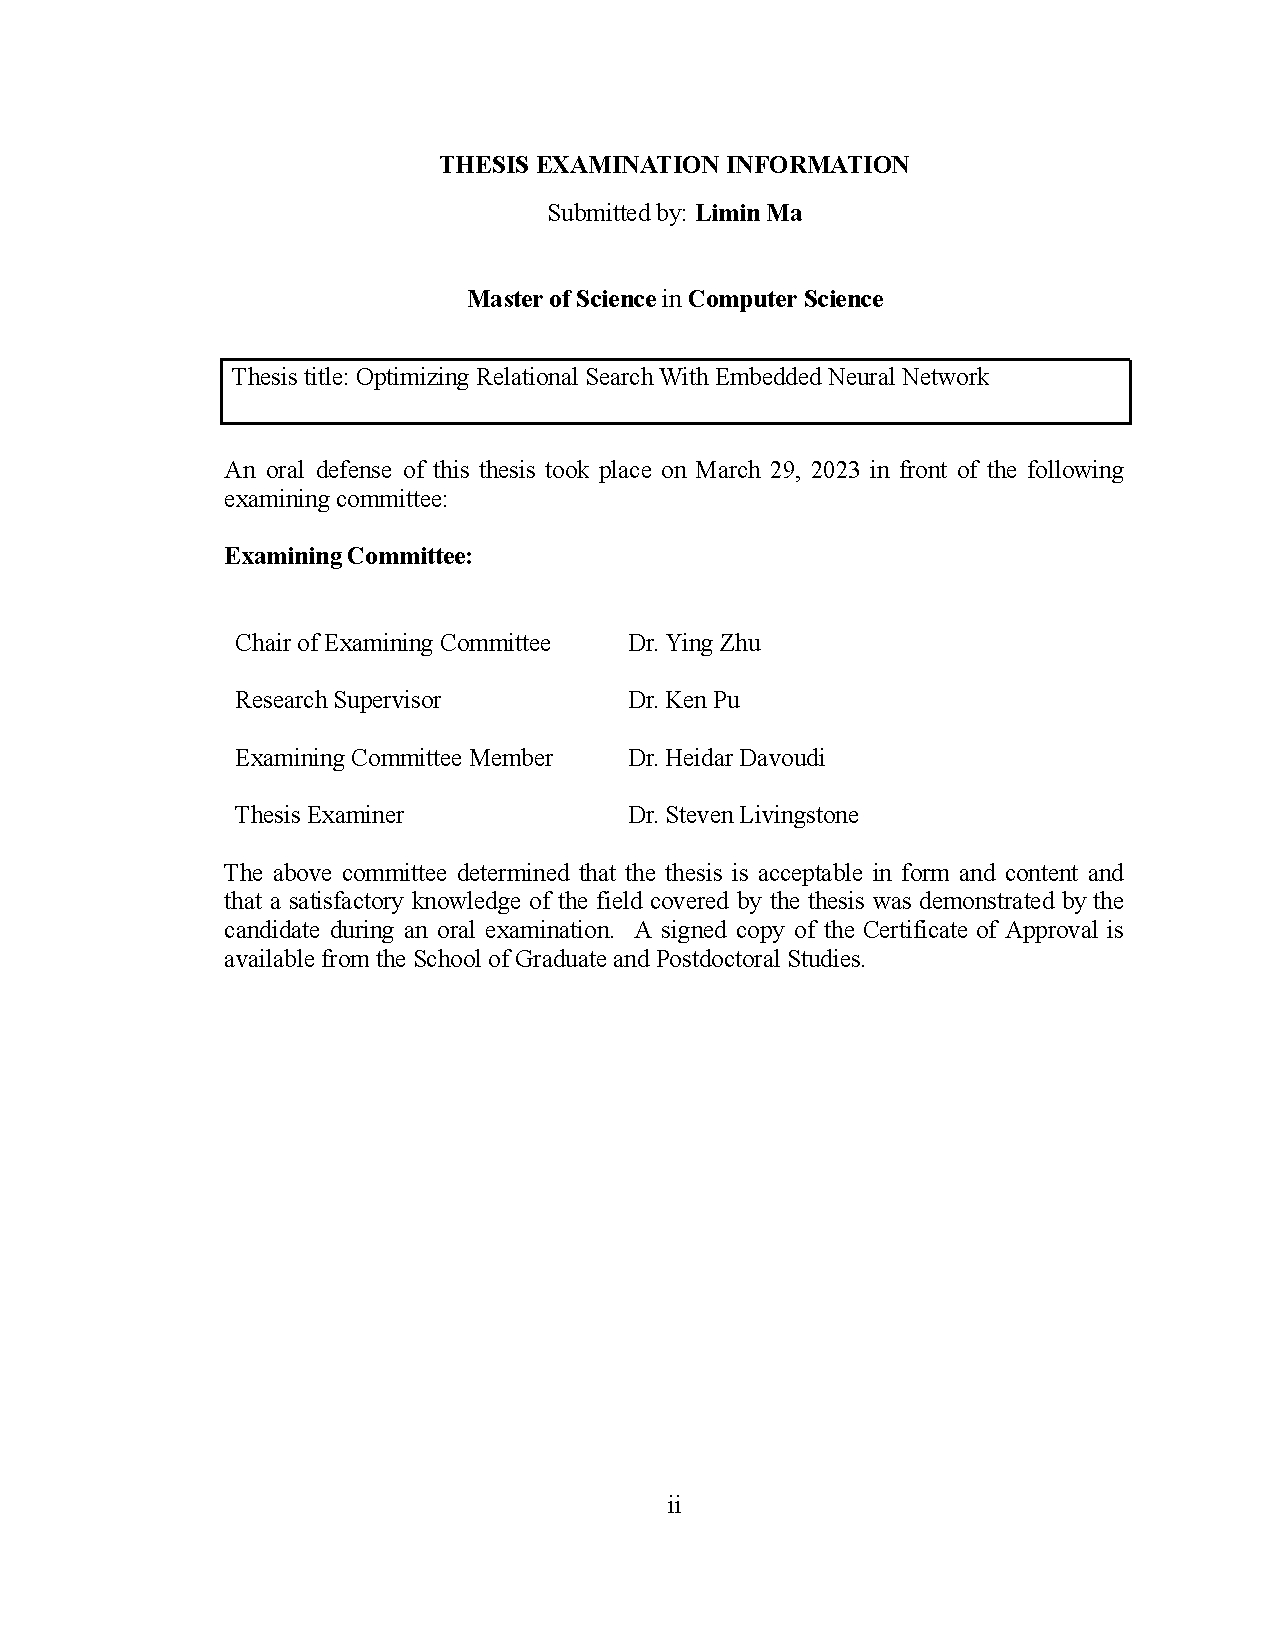
\includepdf{my/exam_info.pdf}
\chapter*{Abstract}
\addcontentsline{toc}{chapter}{Abstract}

Our research focuses on a novel method to query relational data. We propose the partial tuple search problem where a user can utilize keyword search to explore complex relational datasets. The challenge of evaluation of partial tuple queries is the performance bottleneck of fuzzy string matching using traditional full-text index structures. We propose a solution to overcome the bottleneck by incorporating horizontally partitioned full-text indexes and an embeddable neural network classifier in the query processing pipeline. The classifier is trained with self-supervision. It learns to optimize the partitioned indexes access pattern to accelerate query performance. Using textual features of user queries, the classifier infers the index access pattern so that fuzzy string matching subqueries are efficiently evaluated. We studied various network architectures and evaluated them against real-world datasets. Our experimental evaluation demonstrates that neural networks successfully learned how to optimize index access patterns for this use case.
\newline

\noindent{\textbf{Keywords:}} neural network; relational database; keyword search; optimization

\chapter*{Author’s Declaration}
\addcontentsline{toc}{chapter}{Author’s Declaration}

I hereby declare that this thesis consists of original work of which I have authored. This is a true copy of the thesis, including any required final revisions, as accepted by my examiners.

I authorize the University of Ontario Institute of Technology (Ontario Tech University) to lend this thesis to other institutions or individuals for the purpose of scholarly research. I further authorize University of Ontario Institute of Technology (Ontario Tech University) to reproduce this thesis by photocopying or by other means, in total or in part, at the request of other institutions or individuals for the purpose of scholarly research. I understand that my thesis will be made electronically available to the public.

\vspace{3cm}

\noindent \underline{\hspace{8cm}} \hspace{1cm} Limin Ma

\chapter*{Statement of Contributions}
\addcontentsline{toc}{chapter}{Statement of Contributions}

Part of the work described in Chapter 3 has been published as:
\newline

\noindent L. Ma and K. Q. Pu, ``Neural Network Accelerated Tuple Search For Relational Data,'' 2022 IEEE 23rd International Conference on Information Reuse and Integration for Data Science (IRI), San Diego, CA, USA, 2022, pp. 81-82, doi: 10.1109/IRI54793.2022.00029.
\newline

I performed the majority of design, implementation, experimental evaluation and preparation of the manuscript.

\chapter*{Acknowledgements}
\addcontentsline{toc}{chapter}{Acknowledgements}

I would like to express my utmost gratitude to my supervisor, Dr. Ken Pu, for
his guidance, encouragement and support. 
I would also like to thank my committee members, Dr. Heidar Davoudi and
Dr. Steven Livingstone. I am grateful for their valuable feedback on this thesis.
Last but not least, I am thankful to my wife Xiao Wang and the rest of my family.
All have provided me with patience and support for the challenges I faced
in order to perform research and write this thesis.
None of this would have been possible without their support.


% Include lists in singlespacing
\onehalfspacing
\tableofcontents
\listoftables
\listoffigures

\nomenclature{\textbf{API}}{Application Programming Interface}
\nomenclature{\textbf{Conv1D}}{1D Convolution}
\nomenclature{\textbf{CNN}}{Convolutional Neural Network}
\nomenclature{\textbf{CSV}}{Comma-Separated Values}
\nomenclature{\textbf{GPU}}{Graphics Processing Unit}
\nomenclature{\textbf{LSTM}}{Long Short-Term Memory}
\nomenclature{\textbf{ML}}{Machine Learning}
\nomenclature{\textbf{MLP}}{Multilayer Perceptron}
\nomenclature{\textbf{NER}}{Named Entity Recognition}
\nomenclature{\textbf{NLP}}{Natural Language Processing}
\nomenclature{\textbf{OOV}}{Out-Of-Vocabulary}
\nomenclature{\textbf{RDBMS}}{Relational Database Management System}
\nomenclature{\textbf{RNN}}{Recurrent Neural Network}
\nomenclature{\textbf{SQL}}{Structured Query Language}
\nomenclature{\textbf{TF–IDF}}{Term Frequency-Inverse Document Frequency}

\printnomenclature 

\clearpage
\doublespacing
\pagenumbering{arabic}

\mainmatter
\chapter{Introduction}

\section{Motivation}

For many decades, with the availability of low cost computers and Internet access, the amount of digital information or data has increased at an ever growing pace. This poses a challenge to managing information reliably and efficiently. 
%we have been creating, archiving and organizing digital information

Various database technologies and query processing engines have been developed over the past several decades to meet the appetite of information management. There are two main types of databases, relational database and non-relational database. Relational database management system (RDBMS)  is a pillar of database technology. MySQL and PostgreSQL are two examples of open source RDBMS. Examples of non-relational databases include semi-structured databases such as MongoDB \cite{mongodb} and graph databases such as Neo4j \cite{neo4j}. 

In contrast to its peers, RDBMS is proven to be the preferred choice for most of the data management needs.  There are several reasons:

\begin{itemize}
 \item Relational databases help businesses' utilization of data by maintaining data in a simple and efficient way. 
 The relational data model is simple, easy to use and type-safe.
 Relational databases are typically capable of handling transactions, which is often required by businesses.
 The schema management features of RDBMS are robust enough to accurately model business and application requirements, and yet at the same time, provide a rich set of constraints and data consistency checks.  Thus, RDBMS provides a higher level of data consistency.

 \item The Structured Query Language (SQL) is the standard programming language for managing data in relational databases. SQL has been the de facto industry standard for data analysis for several decades, and is still the most widely used method. It can quickly and efficiently process queries with the help of highly optimized SQL engines. It does not require extensive coding and programming skills, and offers users an interactive interface with underlying databases.

 \item Storing data using relational format is the safest choice when facing with the risks of digital data decay and software incompatibility issues.
 RDBMSes are widely used in various applications including mobile apps, Web services, distributed computing clusters, etc. because they offer robust data management capabilities. Combined with SQL's portability, 
 RDBMS and SQL provide the most readily available software compatibility.
\end{itemize}

The dominance of RDBMS started to be challenged by the rise of the World Wide Web. The default mode of content creation on the World Wide Web is textual data and unstructured data. Such content apparently lacks relational structures. Therefore, it is unnatural to fit such data into RDBMS systems. Consequently, SQL is no longer the most suitable language to express queries over textual and unstructured data.

The need to carry out web searches gave the birth of search engines. Search engines started to popularize key-value stores as a preferred choice of data storage, and keyword search as a preferred choice for data retrieval.  As modern search engines demonstrated, keyword search is a surprisingly effective approach of data retrieval. Furthermore, highly scalable and performant full-text indexes, such as Apache Lucene, are available to support keyword search queries at scale. But at the same time, keyword search has limitations that can not be ignored. Primarily, keyword search does not offer ways to reason over a data schema, and thus does not offer the end users ways to easily provide relational joins, selection over predicates or data analytics.

In attempts to overcome the limitations of keyword search while preserving its advantages, many researchers have proposed hybrid query languages that share features of SQL and keyword search.  Most of the proposed systems extend SQL with keyword search, and use a relational database as data storage. While such systems do address the limitations of both SQL and keyword search over relational data to some extent, a common issue is scalability. The performance bottleneck is the inefficiency of relational database indexes when used for full-text search.

In this thesis, we are motivated by the following questions:

\begin{itemize}
\item Can we extend keyword search queries to enhance their expressive power when the underlying data is relational?

\item Can we utilize full-text indexes that are designed for keyword search to answer searching of relational data?

\item What are different ways to optimize the evaluation of keyword search queries?
\end{itemize}

\section{Machine Learning}

The rise of machine learning in recent years was due to two major factors, the explosion of data and the ever more affordable computing power. The ubiquitousness of Internet created the explosion of data that machine learning can consume, and cheap computing resources made it possible to train machine learning algorithms using large amounts of data. Machine learning has found successful applications in almost every corner of computer science and engineering.  The most prominent tool in machine learning is neural networks.  Complex neural network architectures have been designed and trained to perform various tasks at near-human or superhuman levels. One example is AlphaGo, which is a computer program that plays the board game Go. It grabbed the world's attention by defeating a Go world champion in 2016 \cite{alphago}. 

What is particularly amazing about machine learning's success is how widely neural network approaches can be applied, ranging from images to texts, from semantic understanding to content generation.

The best aspects of applying neural networks as part (or whole) of a solution are:

\begin{itemize}

\item Neural networks are more robust than deterministic and combinatorial algorithms.  Given when the input to the network deviates from expectation, the network can complete the processing in a continuous fashion, often producing near optimal results.

\item Neural networks can be much faster during inference mode.  Since neural networks essentially involve only matrix based numerical operations, they are well suited for modern CPUs and general purpose GPUs.  In contrast, traditional algorithms utilize more complex data structures which often require large amounts of random memory access, making them difficult to optimize at the CPU / GPU level.

\item Neural networks are easier at design time.  Machine learning approaches shift the solution complexity from algorithmic design to data collection.  When designing a neural network, we are essentially choosing the right black box that fits the overall system the best.  The challenge is not to design the internal parameters of the black box, but rather to gather sufficient data to evaluate the quality of different candidate blackboxes.  It's been repeatedly demonstrated in the domains including but not limited to image processing, natural language processing and combinatorial games, neural networks with simple architectures (but large number of parameters) outperform sophisticated handcrafted algorithms.
\end{itemize}

Traditionally, network based approaches require the availability of a large corpora of training data.  Often this requires either expensive data collection schemes or human manual labeling of data.  But in situations where training data is not available, it is still possible to apply neural networks.  Self-supervised learning and reinforcement learning are just two examples of training neural networks without prior labeled training data.

While our research objective is novel keyword queries of relational databases, we are particularly motivated to incorporate neural networks into our query processing pipeline in a self-supervised manner.  Towards this goal, we will need to

\begin{itemize}
\item identify problems that can be solved using self-supervised neural networks.
\item design neural networks and incorporate them into the query processing pipeline.
\end{itemize}

\section{Overview of thesis}

The problems we address in this thesis are:

\begin{itemize}
\item extension of keyword search queries over relational data in ways that we can still enjoy efficient query evaluation using full-text indexes.

\item identify components in the query evaluation pipeline that can be optimized by self-supervised neural networks.
\end{itemize}

Towards the first problem, we proposed a novel relational search problem we call {\em partial tuple search}.  It is a generalization of keyword search by allowing users to specify {\em partial tuples} as queries, which can have both value-based keywords and schema-based structure information.  Partial tuples can be used for information retrieval when users have limited, but nonzero, knowledge over the schema of the underlying relational database.

We demonstrate that a partial tuple search query can be evaluated in a pipeline consisting of the following stages:

\begin{itemize}
\item Generating a keyword query from a partial tuple.
\item Evaluating the keyword query using one or more full-text indexes.
\item Completing the partial tuple by matching keyword search results with the partial tuple.
\end{itemize}

It is well known that fuzzy string matching is generally more expensive to evaluate keyword search queries.  In our use case, when we perform fuzzy partial tuple search, the full-text index becomes the performance bottleneck.  A solution is to partition the full-text index, and perform fuzzy keyword search over multiple partitions.  This creates a query optimization opportunity: a well selected index access pattern can speed up the keyword search performance without the additional burden of parallel CPU load.

We have designed neural networks that can learn from the relational data to optimize index access patterns.  The neural network performs classification based on features from textual data in the relational database.  Using the classification probability we can optimize index access patterns so that search time is minimized.
%Our experimental evaluation shows that transformer based networks can achieve optimal index access well over 90\% of the times.



\chapter{Background}

% \begin{itemize}
    \item Provide background material for the partial tuple search, and its solution.  We introduce mathematical notations.
    \item Relational model: table, attributes, tuples, values
    \item Document model: text fields
    \item Document search: tokenization, inverted index
    \item Fuzzy matching with ngram
    \item Existing software libraries: Lucene
    \item Neural language models and embedding vectors
\end{itemize}

Summarize how they are related to the contribution of this thesis.
\section{Relational Data Model}
We describe the relational data model in this section. It is the foundation of the search problem that is studied in this thesis.  

Let $R$ be a relation and $\Attr(R)$ be the attributes of $R$. The attributes are a set of names.  Each tuple of $R$ is
a function that maps attributes of $R$ to values:
$$
t : \Attr(R) \to \Values
$$
The relation $R$ is a set of such tuples:
$$
R = \{t_1, t_2, \dots, t_n\}
$$

\begin{example}
Consider a table shown below:
\begin{center}
    \centering
    \begin{tabular}{|c|c|}\hline
    {\bf Name} & {\bf Address} \\ \hline
    Jack & 100 Simcoe Street \\ \hline
    Jill & 56 Taunton Road \\ \hline
    Joe & 5 Collin Road \\ \hline
    \end{tabular}
\end{center}
The attributes are:
$$ \Attr(R) = \{\mathrm{Name}, \mathrm{Address}\} $$
The relation consists of three tuples:
$$ R = \{t_1, t_2, t_3\} $$
where $t_1$ is a mapping given by:
$$
t_1 = \left[\begin{array}{rcl}
\mathrm{Name} & \mapsto & \makebox{Jack} \\
\mathrm{Address} & \mapsto & \makebox{100 Simcoe Street} \\
\end{array}\right]
$$
The other two tuples, $t_2$ and $t_3$, are defined similarly.
\end{example}

A relational database will have more features added to its relational model. For example,
\begin{itemize}
    \item Primary keys and foreign keys
    \item Dependencies and constraints
    \item Structured query language (SQL)
\end{itemize}
More details can be found in texts such as García-Molina et al  \cite{garcia2005database}.  However, in the context of our thesis, we do not rely on these additional features of a relational model.  More precisely, the relational model we focus on is the first normal form \cite{beeri1979computational}.

\section{Document Models}
While the relational model is widely used, it does have limitations. One such limitation is the lack of flexibility of its schema, namely, all tuples of the same relation {\em must} have the same set of attributes.

Text search engines popularized the document model \cite{croft2010search}. It supports schema-less data management.  In the document model, a document is defined as
a mapping from {\em fields} to text values.

\subsection{Documents}
Let $d$ be a document and $\Attr(d)$ be its set of fields. The fields $\Attr(d)$ is a set of names, similar to the attributes of a relation.
The document $d$ is a function that maps fields to text:
$$ d : \Attr(d) \to \mathbf{Text} $$

A document collection is denoted by $D = \{d_1, d_2, \dots, d_n\}$.
It's important to note that a document collection is fundamentally different from a relation, that is, 
\begin{center}
    different documents $d, d'\ (d\not=d')$ can have different fields:
$\Attr(d)\not=\Attr(d')$.
\end{center}

\begin{example} \label{ex2}
Consider three documents in a document collection $D$. The first has two fields: $Name$ and $Address$. It can be denoted as:
$$
d_1 = \left[\begin{array}{rcl}
\mathrm{Name} & \mapsto & \makebox{Jack} \\
\mathrm{Address} & \mapsto & \makebox{100 Simcoe Street} \\
\end{array}\right]
$$

The second has three fields: $Name$, $Occupation$, and $Address$. It can be denoted as:
$$
d_2 = \left[\begin{array}{rcl}
\mathrm{Name} & \mapsto & \makebox{Jack} \\
\mathrm{Occupation} & \mapsto & \makebox{Student} \\
\mathrm{Address} & \mapsto & \makebox{100 Simcoe Street} \\
\end{array}\right]
$$

The third has four fields: $Restaurant\ Name$, $City$, $Rating$, and $Comment$. It can be denoted as:
$$
d_3 = \left[\begin{array}{rcl}
\mathrm{RestaurantName} & \mapsto & \makebox{The Best Grill} \\
\mathrm{City} & \mapsto & \makebox{Oshawa} \\
\mathrm{Rating} & \mapsto & \makebox{5} \\
\mathrm{Comment} & \mapsto & \makebox{very nice place} \\
\end{array}\right]
$$
\end{example}

\subsection{Tokenization}

The main objective of the document model is to support keyword search efficiently.  This involves searching for documents whose fields contain certain sub-strings, which we call {\em tokens}.  The process of token generation is referred to as tokenization (also known as lexical analysis).  Tokenization is an important step in natural language processing \cite{jimenez2018impact,kudo2018sentencepiece}, especially for non-English languages \cite{takaoka2018sudachi,cao2011research}.

Before we can store the documents, we first need to transform text values into lists of tokens.  We do this by using a tokenizer:
$$
\mathbf{tokenize} : \mathbf{Text} \to \List[\Token]
$$

Given a document $d$, a {\em term} is a field-token pair that is derived from the result of tokenzing the text value of a field.
Then the term set of a document $d$ is given by:
$$
\mathbf{termset}(d) = \{
  (f, x): f\in\Attr(d),\ x\in\mathbf{tokenize}(d(f))
\}
$$

Given a document collection $D$, a simple document query is to find all documents with a specific term: $term^* = (f^*, x^*)$.  The answer set to the query is given as:
$$\mathbf{answerset}(D, term^*) = \{d\in D: term^*\in\mathbf{termset}(d)\}$$

\begin{example}
Consider the above three documents in the document collection $D$ of Example \ref{ex2}. If we search field ``Address" by keyword ``Simcoe", the search query is:
$$term^* = (Address, Simcoe)$$. 
The answer set will be:
$$\mathbf{answerset}(D, term^*) = \{d1, d2\}$$

\end{example}

\subsection{Keyword queries and matching scores}

Internet search engines made keyword queries as a standard way of accessing text documents \cite{ntoulas2004s}.
Important aspects of keyword queries are:
\begin{itemize}
    \item There is no fixed syntax: queries can be as simple as a phrase or a piece of plain text.
    \item The search results do not need to match the query perfectly. They are ranked by some matching scores instead.
\end{itemize}

A {\em keyword query} is a text, annotated by a field name.
$$Q = (f_q, q)$$
where $f_q$ is a field name, and $q\in\mathbf{Text}$.

The matching between the query $Q = (f_q, q)$ and the documents in a collection $D$ is determined by the matching of their respective termsets.  The termset of the query is defined as:
$$
\mathbf{termset}(Q) = \{(f_q, x): x\in\mathbf{tokenize}(q)\}
$$

\newcommand{\Termset}{\mathbf{termset}}
\newcommand{\TFIDF}{\mathbf{TFIDF}}
A natural matching score between $Q$ and some document $d$ is the overlap between their termsets.  The Jaccard similarity measures a normalized overlap as defined as:
$$
\mathrm{sim}(Q, d) = \frac{|\Termset(Q)\cap\Termset(d)|}{|\Termset(Q)\cup\Termset(d)|}
$$

Jaccard similarity is sufficient in many document retrieval scenarios. However, it is not the ideal measure for documents based on natural languages. There are many words in the vocabulary of natural language text that have overwhelming high frequencies, for example, {\em the}, {\em a}, {\em this}, etc.  Their occurrences should be discounted towards the similarity score.  {\em Term frequency-inverse document frequency} (tf-idf) measure is a term-normalized score better suited for natural language based query-document matching.

Each term $t\in\Termset(d)$ in a document $d$ has a weight, known as its tf-idf weight, defined as follows.

Denote the number of occurrences of $t$ in $d$ as $\#(t,d)$.  The term frequency is the normalized number of occurrences of $t$:
$$
\mathrm{TF}(t, d) = \frac{\#(t, d)}{\sum_{x\in\Termset(d)}\#(x, d)}
$$
In order to discount frequent words, we also compute the {\em inverse document frequency} of $t$ with respect to the entire document collection $D$:
$$
\mathrm{IDF(t)} = \log \frac{|D|}{|\{d\in D: t\in\Termset(d)\}|}
$$
Note that $\mathrm{IDF}(t)$ is inversely proportional to the popularity of a word.  Frequently occurring words have lower IDF weights.

Finally, the TF-IDF weight is the produce:
$$
\TFIDF(t, d) = \mathrm{TF}(t, d)\cdot \mathrm{IDF}(t)
$$

If a term $t$ does not appear in a document $d$, then its TF-IDF weight is zero.  Each document and query can be seen as a (sparse) vector of TF-IDF weights, and their matching score is measured by the cosine similarity of their TF-IDF vector representation.
\begin{equation}
\mathrm{sim}(Q, d) = \frac{\sum_{x}\TFIDF(x, Q) \TFIDF(x,d)}{
\sqrt{\sum_{x}\TFIDF(x,Q)^2 \sum_{y}\TFIDF(y,d)^2}
}
\label{eq:tfidf-sim}
\end{equation}

Equation~\ref{eq:tfidf-sim} provides an unbiased measure of similarity between the termsets of the query and a document by discounting frequently occurring words.

\section{Document Indexes and Search Engines}
In the previous section, we have defined a number of similarity measures which can be used to rank {\em all} documents with respect to a user defined query.

A search engine needs to efficiently identify the top-$k$ matching documents using some similarity score.  A naive approach would require evaluating the similarity score of all the documents, which has a data complexity of $\mathcal{O}(n)$, where $n$ is the total number of documents.  For large document corpora, search engines need better algorithms for keyword query processing.

\newcommand{\Id}{\mathbf{id}}
\newcommand{\Idset}{\mathbf{idset}}

The most widely used data structure for keyword search is the {\em inverted term index}. 
Let $D$ be a document collection. The term set of $D$ is given by,
$$
\Termset(D) = \{\Termset(d):  d \in D\}
$$
Let $\Id(d)$ be the id of a document $d$. The inverted term index is a function mapping terms to lists of document ids,
$$
\mathbf{index} : \Termset(D) \to \List[\Id(d): d \in D]
$$

\begin{example}
Consider the three examples in Example \ref{ex2}. The inverted term index can be denoted as,
$$
\left[\begin{array}{rcl}
	\mathrm{(Name, Jack)} & \mapsto & \makebox{\{d1, d2\}}  \\
	\mathrm{(Address, 100)} & \mapsto & \makebox{\{d1, d2\}}  \\
	\mathrm{(Address, Simcoe)} & \mapsto & \makebox{\{d1, d2\}}  \\
	\mathrm{(Address, Street)} & \mapsto & \makebox{\{d1, d2\}}  \\
	\mathrm{(Occupation, Student)} & \mapsto & \makebox{\{d2\}}  \\
	\mathrm{(RestaurantName, The)} & \mapsto & \makebox{\{d3 \}}  \\
	\mathrm{(RestaurantName, Best)} & \mapsto & \makebox{\{d3 \}}  \\
	\mathrm{(RestaurantName, Grill)} & \mapsto & \makebox{\{d3 \}}  \\
	\mathrm{(City, Oshawa)} & \mapsto & \makebox{\{d3\}}  \\
	\mathrm{(Rating, 5)} & \mapsto & \makebox{\{d3\}}  \\
	\mathrm{(Comment, very)} & \mapsto & \makebox{\{d3\}}  \\
	\mathrm{(Comment, nice)} & \mapsto & \makebox{\{d3\}}  \\
	\mathrm{(Comment, place)} & \mapsto & \makebox{\{d3\}}  \\
\end{array}\right]
$$
\end{example}

\subsection{Keyword query performance}
Inverted term index \cite{putz1991using}, as illustrated in Figure \ref{fig:inverted_term_index}, has two main components: a dictionary and lists of document ids.
\input{my/chapters/background/figures/inverted-term-index.tex}
We use the dictionary to look up a search term. After that, we retrieve the list of document ids associated with the term. Therefore, the query performance is determined by looking up terms of the query in the dictionary and merging all matched document id lists.

Let $q = <t_1, t_2, \dots, t_k>$ be a query, where $t_i$ are terms and $k$ is the number of terms of the query. The average length of document id lists is denoted as $l$. The total number of terms in the inverted index is denoted as $N$. Looking up a term $t_i$ has $\mathcal{O}(\log N)$ complexity. Merging matched document lists requires linear scan, which has $\mathcal{O}(k \times l)$ complexity . Therefore, the time complexity of processing the query is $\mathcal{O}(k \times \log N) + \mathcal{O}(k \times l)$.

\subsection{Fuzzy string matching and collisions}
\label{sec:fuzzy-collision}
A particularly important feature of keyword search based information retrieval is {\em fuzzy string matching}.  A common practice in performing fuzzy string matching based on the {\em n-grams} of the text \cite{kim1994fast}.

\begin{definition}[n-grams]
Let $s$ be a string where $s(i)$ is the $i$-th character from some alphabet $\Sigma$.  Let $n\geq 1$ be an
integer.  The $n$-padded string of $s$ is obtained by prepending and appending $n-1$ special symbols to $s$, defined as:

$$
s' = \underbrace{\mathtt{'\$'}\dots \mathtt{'\$'}}_{n-1\ \mathrm{times}} \cdot s\cdot
\underbrace{\mathtt{'\$'}\dots \mathtt{'\$'}}_{n-1\ \mathrm{times}} 
$$

The $n$-gram of $s$ is the set of strings of length $n$ defined as:
$$
\mathrm{G}_n(s) = \{s'(i) \dots s'(i+n-1): 1\leq i\leq |s'|-n+1\}
$$
\end{definition}

By definition, $G_n(s)\subseteq(\Sigma\cup\{\$\})^n$, namely all of its segments of length $n$ including
the padded special character $\$$.

\begin{example}
    Suppose that $s = \mathtt{``computer''}$.  Its 3-grams are given as:
    $$
    G_3(s) = \{
    \mathtt{\$\$c, \$co, com, omp, mpu, put, ute, ter, er\$, r\$\$}
    \}
    $$
\end{example}

Since $G_n(s)$ is a set that is derived from the content of $s$, we can
use it as a feature to compare strings in an approximate way.

\begin{definition}[Jaccard Similarity]
    Given two sets $A$ and $B$, their Jaccard similarity
    is given by:
    $$ J(A, B) = \frac{|A\cap B|}{|A\cup B|}$$

    Note $0\leq J(A, B)\leq 1$, with $J(A, B) = 1$ if and only if $A=B$.
\end{definition}

Using Jaccard similarity (and its derivatives), we can introduce
a similarity measure over strings.  Given two strings $s_1$ and $s_2$, the Jaccard similarity of the two strings is given by:
$$ J(s_1, s_2) = J(G_n(s_1), G_n(s_2)) $$

Now we can perform fuzzy string search using Jaccard similarity over strings. We index documents by storing their n-gram sets. The inverted index, therefore, will have n-gram tokens.
We also break all queries into n-gram sets for searching. Commonly 3-grams yield the best trade-off for the English language.

Recall that the inverted term index maps tokens to documents.  When 3-gram tokens are used, the total possible number of distinct tokens are given by
$|\Sigma|^3$. For the English language, $|\Sigma|\simeq 50$ (based on ASCII encoding).  So, there will only be $50^3 = 125,000$ possible tokens.  But, at the same time, a typical text index needs to support up to billions of documents.  As the number of documents exceeds the number of possible tokens, we run into the bad situation of severe collisions, which degrades the performance
from log-time $\mathcal{O}(\log n)$ to sequential scan $\mathcal{O}(n)$.

In this thesis, we will encounter the bottleneck of collision when 3-grams are used as tokens.  We will study methods involving partitioning the index, and optimizing index access pattern so that the search speed is improved.  Our optimization method will involve neural networks to learn the optimal access patterns using self-supervised learning.

In subsequent sections, we will review some elements of neural network design that are necessary to construct our embedded networks.

\section{Learning with neural networks}
\label{sec:neural-networks}
A neural network allows us to find patterns based on its training data. A trained neural network is an approximation of a function that maps its input data to its output data. In the context of this thesis, we explore ways to design neural networks as classifiers that will map partial tuple search queries to the relations that contain the tuples.


\subsection{General framework of machine learning}

The general framework of machine learning consists of three main components: representation of training data, a trainable model, and an optimization algorithm \cite{lecun2015deep,bengio2017deep}.

There are different types of data that can be used for machine learning, such as numerical data, text documents, images, and so on. They have to be converted to some format before they can be consumed by a machine learning model. In natural language processing, we use embedding vectors, which are numerical vectors, to represent texts \cite{li2018word,tripathy2021comprehensive}.

Fundamentally, the problem that machine learning (ML) is addressing must be modeled as a function:

$$
f : X \to Y
$$
where $X$ is a vector space that is the encoding of the input objects, and $Y$ is the output (usually also a vector space).  In the context of machine learning, the exact form of $f$, either mathematically or computationally, is not available.  However, we assume that we have many observations of the input-output pairs $\{(x_i, y_i): i=1\dots n\}$ of $f$.  The collection of $(x,y)$ pairs is known as the {\em training data}.

A trainable model is an algorithm that can learn from the training data. In the case of a neural network model, we define its structure by layers. We specify the number of layers the model consists of, the layer types, the number of neurons in each layer, and the connections between layers. The network structure determines the capabilities of the model.

We highlight the following  layer architectures that are used in this thesis.

\begin{itemize}
    \item Embedding layer: this layer architecture converts discrete and categorical inputs to dense vectors using a {\em hard coded} lookup table
    that maps tokens from a vocabulary to embedding vectors.  We will discuss this in more detail in Section~\ref{sec:embedding-layer}. The parameters
    of the embedding layer store the lookup table.
    \item Linear layer: this is the layer that is capable of performing linear separation in high dimensional space.  A linear layer is most commonly used
    as a hidden layer or an output layer to produce the intermediate or final logits for a multi-class classification problem.  It has
    a dense connection between the input and output.  Generally, its dense connection makes it unsuitable to capture spatial and sparsely distributed
    features in the input.  The parameters of the linear layer store the matrix and bias used in the linear transformation.
    \item Convolution layer: this layer architecture is designed to address the dense connection problem of the linear layer.  Using the mathematical
    operation known as {\em convolution}, the convolution layer has spare connections between its input and output, and thus can learn localized
    features in the input.  The parameters of the convolution layer store the {\em kernels} used in the convolution.
    \item Recurrent layer: the recurrent layer processes sequential inputs, namely it maintains an internal high dimensional state so that
    its output sequence depends (indirectly) on all previous inputs.  The parameters of the recurrent layer store the matrices (and bias)
    used to update the internal state, and generate the sequential output.
    \item Attention layer: the attention layer is motivated by the inter-input dependencies.  It performs transformation on two sets of input vectors
    by finding dependencies between vectors in one set and those in the other set.  In the case of self-attention, the same set of vectors
    are used as both sets. The parameters of the attention layer store the transformation matrices that combine the two sets of input vectors.
\end{itemize}

A complete model consists of compositions of different layers by connecting the output of one or more layers to the input of downstream layers.
A final output layer produces the output of the model.  The parameters of the model are the collection of the parameters of all layers.

An optimization algorithm is the working force to tune the model.
We define an objective function and use the optimization algorithm to minimize or maximize it. One typical example of an objective function is a loss function. It computes the error between the prediction and the target. Therefore, the goal of model training is to minimize the error. Various optimization algorithms exist, such as gradient descent, least square error minimization, etc. For neural network model training, we can use gradient descent to iteratively update the network weights to minimize the loss.
 
Once the model is trained, we can use it for prediction. A neural network model will process input data through its layers and produce an output, which is the prediction of the model. The quality of the prediction will depend on the quality of the training data, the model's architecture, and the effectiveness of the training process.

In the following sections, we describe embedding layer and specific neural network architectures that we use in our research.

\subsection{Embedding layer}
\label{sec:embedding-layer}
Embeddings are vectors of floating point numbers that can be used to represent various types of data, such as text, images, audio, etc.
In a natural language processing (NLP) system, the embedding layer is a crucial component. It converts words into numerical vectors with fixed dimensions, which are dense representations of texts.

The main advantage of using embedding layers is that they can capture the complex relationships and semantic meanings of words within a language. Traditional NLP techniques often rely on one-hot encoding, where each word is represented by a binary vector with a ``1" in the position corresponding to the word and ``0"s in all other positions. This approach does not account for the semantic or syntactic relationships between words.

In contrast, embedding layers use a continuous vector space where words with similar meanings are clustered together. This allows the NLP model to better understand the context and meaning of words in a sentence, improving its performance on tasks such as sentiment analysis or language translation. Additionally, because embedding layers have fewer dimensions than one-hot encoded vectors, they require less computational resources and can be trained more efficiently.

Let $\mathbf{Voc}$ be a set of categorical values.  Each element $t\in\mathbf{Voc}$ is called a token.  Without loss of generality, we
arbitrarily sort the vocabulary, and thus we can assume $\mathbf{Voc} = \{1, 2, \dots, N\}$ where $N = |\mathbf{Voc}|$.  Thus,
we can assume that each token is a natural number in $[1, N]$.

The embedding layer has a trainable parameter: $E\in\mathbb{R}^{N\times k}$ for some $k>0$.  It maps each possible token $t$
to a $k$-dimensional vector: $E[t]\in\mathbb{R}^k$, which is known as the {\em embedding vector} of the token $t$.

Since all other layers assume vectors as inputs, the embedding layer is almost always used as the input layer to a neural network
that processes discrete values.

\subsection{Multilayer perceptrons}
\label{sec:mlp}
A Multilayer Perceptron (MLP) is a type of neural network with a simple, feedforward architecture. It consists of an input layer, one or more hidden layers, and an output layer. The input layer receives the input data, and each subsequent layer receives the output of the previous layer as input. The output of the final layer is the network's prediction.

MLPs are simple and easy to train, making them a popular choice for many applications. They are also versatile, as they can be used for a wide variety of tasks, including classification, regression, and clustering. Additionally, MLPs are able to learn non-linear relationships, which is not possible with simpler models such as linear regression. This makes them well-suited for many real-world problems where the relationship between the input and output is not strictly linear.

The MLP consists of two linear layers: a hidden layer and an output layer.

\begin{eqnarray*}
f_1 &:& \mathbb{R}^m \to \mathbb{R}^h : x \mapsto \sigma_1(W_1 x+b_1)\\
f_2 &:& \mathbb{R}^h \to \mathbb{R}^n : x \mapsto \sigma_2(W_2x+b_2)
\end{eqnarray*}
where $(W_i, b_i)$ is the transformation matrix and bias vector of layer $i$, and $\sigma_i$ is a non-linear activation function.

MLP is the composition of the two layers:

$$
\mathbf{MLP}(x) = f2(f1(x))
$$

MLPs can be applied to Natural Language Processing (NLP) applications in several ways. One common approach is to use an MLP to classify text documents or sentences according to their content. For example, an MLP could be trained to classify a sentence as positive or negative sentiment, or to categorize it into one of several predefined categories such as sports, politics, or entertainment.

Another way in which MLPs can be used in NLP is for language translation. In this case, the MLP would be trained on a large dataset of sentence pairs in different languages, with the goal of learning to translate a sentence in one language to the corresponding sentence in the other language. The input to the network would be a sentence in the source language, and the output would be the translation in the target language.

\subsection{Sequence learning with recurrent neural networks}
\label{sec:rnn}
Sequence learning is a type of machine learning that trains models to make predictions based on sequential data, such as time series data or natural language texts. Recurrent neural networks (RNNs) are a type of neural network that is very capable of handling sequence learning tasks. This is because they are able to retain information from previous time steps and use it to inform their prediction of the next time step. This allows RNNs to make predictions about data that has dependencies on previous data points, such as the next value in a time series or the next word in a sentence of natural language.

The input of a RNN is a sequence of vectors from $(\mathbb{R}^m)^*$.
An RNN has two inner layers:

\begin{eqnarray*}
    f_S &:& \mathbb{R}^{m} \times \mathbb{R}^{h} \to \mathbb{R}^h \\
    f_O &:& \mathbb{R}^{h}\to\mathbb{R}^n
\end{eqnarray*}

The vector space $\mathbb{R}^h$ is the $h$-dimensional state space,
and $\mathbb{R}^n$ is the $n$-dimensional output space.  The function $f_S$ computes the next state and $f_O$ computes the final output.

Given an input sequence $(x_1, x_2, \dots, x_L)$, and 
an initial $s_0\in\mathbb{R}^h$, we compute a sequence of states $(s_1, s_2, \dots, s_L)$, where
$$
s_i = f_S(x_i, s_{i-1})\ \mathrm{for}\ i\in[1, L]
$$

Thus, for each step $i$, $s_i$ indirectly depends on $x_1, x_2, \dots x_i$.

The final output is given by:
$$
y = f_O(s_L)
$$

We can design $f_S$ and $f_O$ using general vector-to-vector layers (such as MLP).  See the survey \cite{yu2019review} for different design possibilities.  

RNNs can also be ``unrolled" in time to remove cycles from its graph. It can be conceptualized as copying the network for each time step along the input sequence, with the same weights shared. This means that RNNs can process inputs of any length and make predictions at any point in the sequence.  The training of RNN is challenging because unrolling creates numerical challenges to the gradient optimization algorithms.

Generally speaking LSTM (long short term memory) is considered the most numerically effective design to implement an RNN.

\subsection{Convolution in sequence learning}
\label{sec:cnn}
1D convolution is a mathematical operation that takes two input signals and produces a third output signal. In the context of natural language processing (NLP), 1D convolution can be used to process text data. The input signals are typically the words or characters in a sentence, and the output signal is a new representation of the sentence that is more useful for downstream tasks such as sentiment analysis or named entity recognition (NER).

To define the 1D convolution operation, we need to make a few auxiliary definitions.

Consider a sequence of length $L$ of scalar values: $\vec{x} = (x_1, x_2, \dots x_L) \in\mathbb{R}^L$.

\begin{itemize}
    \item {\bf $l$-window}: at each position in the sequence $1\leq i\leq L$, the $l$-window
    is defined as $x_{i}, x_{i+1}, \dots  x_{i+l-1}$.  It is the consecutive sequence from $i$ to $i+l-1$.
    We will denote it as $x[i:i+l-1] \in \mathbb{R}^{l}$.

    \item {\bf Kernel}: a {\em kernel} $K$ is a sequence of length $l$ where $l < L$.

    \item {\bf Convolution}: is a process of generating a sequence of outputs $\vec{y} = (y_1, y_2, \dots y_{L-l+1})$ of length $L-l+1$.  It is given by:
    $$
    y_i = \left<x[i:i+l-1], K\right> = \sum_{j=1}^l x[i+j-1]\cdot K[j]
    $$
    Namely, $\vec y = \vec x * K$.
\end{itemize}

The convolution layer generalizes 1D convolution in two important ways:

\begin{enumerate}
    \item Multidimensional input vectors:  each $x_i$ is a vector in $\mathbb{R}^m$.
    Thus, each $y_i$ is the sum of the scalar convolutions:
    $$
    y_i = \sum_{j=1}^l \left<x[i+j-1], K[j]\right>
    $$
    \item Multiple kernels are used to generate multidimensional output vectors:
    With $n$ kernels $K_1, K_2, \dots K_n$, for each window $i$, we generate:
    $$
    y_i = \left[\begin{array}{c}
    \left<x[i:i+l-1], K_1\right> \\
    \left<x[i:i+l-1], K_2\right> \\
    \vdots \\
    \left<x[i:i+l-1], K_n\right> \\
    \end{array}
    \right]
    $$
\end{enumerate}

Thus, with $n$ kernels, the 1D convolutional layer maps an input sequence of $\mathbb{R}^m$ vectors to an output sequences of $\mathbb{R}^n$ vectors.  The $n$ kernels with window size $l$ are the model parameters.

A complete convolutional neural network (CNN) requires some additional features:

\begin{itemize}
    \item {\bf Non-linear activation function}.  The output $\mathbf{conv}(x, K)$ is processed by
    a non-linear activation function $\sigma$:
    $$ y = \sigma(\mathbf{conv}(x, K))$$

    \item {\bf Padding and pooling}. By default the convolution layer changes the sequence length
    $L$ to $(L-l+1)$.  Padding is to augment the initial sequence with additional $l-1$ special 
    boundary vectors such that the length of convolution output is $L$.  Padding is to preserve the sequence length during convolution.  
    Pooling is to aggregate each $w$-window to a single value.  Thus, pooling with a stride of $w$ is to convert a sequence of length $L$ to \floorbrackets{$L/w$}.
    Together, padding and pooling allows us to fine control the output sequence length of the convolution layer.

    \item {\bf Output linear layer}.  The final output of the CNN is a probability distribution
    of $p\in\mathbb{R}^c$ if we are to perform a $c$-category classification task.  A linear layer is used
    to convert \floorbrackets{$L/w$}$\times n$ output from the convolution/pooling layer to size $c$.
\end{itemize}

\subsection{Attention and transformer models}
\label{sec:transformer}
Attention is a mechanism used in some neural networks to allow a model to focus on certain parts of its input. This allows the model to handle inputs of variable length and to learn to weight different parts of the input differently. For example, in natural language processing (NLP), attention mechanism can be used to allow a model to focus on certain words in a sentence to better understand its meaning.  

Given a finite set of vectors, $X = \{x_1, x_2, \dots x_n\}\subseteq\mathbb{R}^m$, the (self) attention layer processes all the vectors in $X$ simultaneously: 
$$
(y_1, y_2, \dots y_n) = \mathbf{Attention}(x_1, x_2, \dots, x_n)
$$
where each input vector $x_i$ is transformed to its respective attended output $y_i$.  The output $y_i$
should capture information about $x_i$ {\em augmented} by other input vectors that $x_i$ {\em attends} to.
For example, if $\{x_i\}$ forms a sequence, then it's possible for $x_i$ to pay attention to 
its immediately adjacent vectors $\{x_{i-1}, x_{i+1}\}$.  The attention layer dynamically computes
the attention and the attended output for {\em each} input vector $x_i$.

The attention is modeled by a $n\times n$ matrix of attention scores:

$$
a_{ij} = \mathbf{AttentionScore}(x_i, x_j)\in[0, 1]
$$

A popular approach to compute the attention score is to learn latent representations known as keys and queries of each $x_i$ using simple linear layers:

\begin{itemize}
    \item $k_i = W_1 x_i + b_1 \in\mathbb{R}^d$
    \item $q_i = W_2 x_i + b_2 \in\mathbb{R}^d$
\end{itemize}

The key and query vectors belong to the same vector space, and their scaled inner products
give us the attention score:

$$
a_{ij} = \mathrm{softmax}_{j}\left(\frac{\left<q_i, k_j\right>}{\sqrt{d}}\right)
$$

Finally, the attended output $y_i$ is the linear combination of $\{x_i\}$ with the attention scores
as the mixture coefficients:

$$
y_i = \sum_j a_{ij}x_i
$$

Transformer models are based on neural network architectures that use attention mechanisms extensively. The original transformer model was introduced in a paper by Vaswani et al. \cite{DBLP:journals/corr/VaswaniSPUJGKP17} in 2017. It was considered a major advance in the field of NLP, and since then various transformer-based models have appeared and been widely used in NLP tasks. Transformer models are notable for their ability to process input sequences in parallel, which makes them much faster to train and evaluate than other models.


\subsection{MLP Mixer}
\label{sec:mlp-mixer}
MLP Mixer \cite{tolstikhin2021mlp} is a neural network that processes multi-channel inputs in two stages: token mixing followed by channel mixing.

The input to a MLP mixer is a fixed-length sequence of feature vectors:

$$\vec x = (x_1, x_2, \dots, x_L)$$
where each $x_i\in\mathbb{R}^C$, and $L$ is the length of the sequence. $C$ is the number of channels.  Each $x_i$ is a feature
of a token consisting of $C$ channels of scalars.  Collectively we have $\vec x\in\mathbb{R}^{L\times C}$.

In order to explain token mixing and channel mixing, we need to introduce the notation of {\em distributed} function application first.

Suppose we have two functions, 
$f: \mathbb{R}^m\to\mathbb{R}^m$ and $g:\mathbb{R}^L\to\mathbb{R}^L$.
Given a matrix $X \in\mathbb{R}^{L\times m}$, its column vectors are in $\mathbb{R}^L$, and its row vectors are in $\mathbb{R}^m$.  Therefore, we can apply $f$ to row vectors, and $g$ to column vectors.
This creates two possible outputs by {\em distributedly} applying $f$ and $g$.

\begin{eqnarray*}
U[i, :] &=& f(X[i, :])\ \mathrm{for\ all}\ i\in[1, L] \\
V[:, j] &=& g(X[:, j])\ \mathrm{for\ all}\ j\in[1, m]
\end{eqnarray*}

In MLP mixer, the input $\vec x$ will be processed by two separate MLPs: the first MLP is distributed along
its tokens (token mixing), and then the second MLP is distributed along the channels (channel mixing).  The MLP mixer mixes the output of the two mixing MLPs back to the original feature vectors.

The first stage, token mixing, produces the output defined by:

$$
U[:, j] = \vec x[:,j] + W_2\sigma(W_1\vec{x}[:,j])
$$
where $W_1, W_2$ are the matrices of the first MLP.

The second stage, channel mixing, produces the output by distributing the second MLP:
$$
Y[i,:] = U[i,:] + W_4\sigma(W_3 U[i,:])
$$
where $W_3, W_4$ are the matrices of the second MLP.

The mixing MLPs do not use any bias vectors.

As demonstrated \cite{tolstikhin2021mlp}, MLP mixer exhibits many desirable qualities
such as faster training time for very large training datasets, smaller model size when compared to very large computer vision models, and finally its performance is nearly and sometimes exceeds state-of-the-art models in many vision tasks.



\chapter{Search Algorithm and Neural Network Accelerated Indexing}

In this chapter, we define our problem and present our proposed solution.

\noindent{\bf Problem statement:} We want to extend keyword search to relational data using full-text index with the help of an embeddable neural network that optimizes the query processing pipeline. 
Given a relational database consists of $K$ relations $R_1, R_2, R_3, \dots, R_K$, the goal is to build a system that takes a partial tuple as user query and can find an optimally matching complete tuple $\vec r \in R_i$ ($i \in \{1, 2, \dots, K\}$) efficiently.

\section{Problem definition of partial tuple search}
In this section, we provide some definitions related to partial tuple search.
Let $R$ be a relational table.  Recall that $\Attr(R)$ is the attributes of $R$, and tuples in $R$ are mappings from $\Attr(R)$ to $\Values$.

\begin{definition}[Labeled values and partial tuple]
Let $R$ be a relational table.  A labeled value in $R$ is a pair $(l:x)$ where 
$l\in\Attr(R)\cup\{?\}$ and $x\in\Values$.  A partial tuple $\vec{x}$ is a set of labeled values: $\vec x = \{(l_i, x_i): i\in I\}$.  We define the attributes of a partial tuple $\vec x$ as the labels of the partial tuple:
$$\Attr(\vec x) = \{l_i\}_{i\in I}$$.
A partial tuple is considered {\bf\em complete} if $\Attr(\vec x) = \Attr(R)$.
\end{definition}

We will write $\vec x[l_i]$ to denote the corresponding value $x_i$.

Note that a partial tuple is a set of values and their respective attribute names from a relational table.  However, we allow a special symbol ``$?$" to be in place of the attribute name.  The special attribute ``$?$" indicates that the attribute name is unspecified (or unknown). The following example illustrates two partial tuples. The second partial tuple has a wild card ``?" as its attribute name:

\begin{example}
\begin{eqnarray*}
\vec s_1 &=& \{\mathrm{name}:\mathrm{Einstein}\} \\
\vec s_2 &=& \{\mathrm{name}:\mathrm{Einstein},\ \mathrm{?}: \mathrm{Professor}\}
\end{eqnarray*}
\end{example}

A query is a partial tuple: $\vec Q = \{(l_i, q_i): i\in I_Q\}$.  The values $q_i$ are keyword queries.
We want to find a complete tuple $\vec r \in R$ that matches $\vec Q$ optimally.  This requires us to define how to compare the partial tuple $\vec Q$ with a complete tuple $\vec r$.  The guiding principle of comparing the two tuples is to match labeled values from $\vec Q$ with those from $\vec r$ according to the following:
\begin{itemize}
    \item Match the labels if they are not the wild card ``$?$".
    \item Match the values using a fuzzy string matching score.
    \item Optimize the sum of similarities between labeled values from $\vec Q$ and those from $\vec r$.
\end{itemize}
Towards this end, we define the following similarity measures:

\begin{definition}[Similarity of labeled values]
\label{def:sim-labeled-values}

Consider two labeled values: $(l_1: x_1)$ and $(l_2, x_2)$,
where $l_1$ and $l_2$ are two labels from $\Attr(R)\cup\{?\}$.  The similarity between the two labels $l_1$ and $l_2$ is given by:
    $$
    \Sim(l_1, l_2) = \left\{
    \begin{array}{cl}
    1 & \mathrm{if}\ l_1 = l_2\ \mathrm{and}\ l_1\not=?,\ l_2\not=? \\
    0 & \mathrm{if}\ l_1 \not= l_2 \ \mathrm{and}\ l_1\not=?,\ l_2\not=? \\
    0.5 & \mathrm{if}\ l_1 = ?\ \mathrm{or}\ l_2 = ?
    \end{array}
    \right.
    $$
    Thus, whenever $l_i$ is the wildcard `` $?$", the similarity is 0.5. Otherwise, it is determined by the equality comparison of the two labels.

The similarity between the two values $x_1$ and $x_2$ is based on string comparison.  We utilize
the Jaccard similarity between the 3-grams of $x_i$:
$$
\Sim(x_1, x_2) = \mathrm{Jaccard}(\mathrm{3grams}(x_1), \mathrm{3grams}(x_2))
$$

Finally, the similarity of the two labeled values is computed as the product of the
similarity between labels and similarity between values.
$$
\Sim((l_1:x_1), (l_2,x_2)) = \Sim(l_1, l_2)\cdot\Sim(x_1, x_2)
$$
\end{definition}

Recall that the user query is a partial tuple $\{(l_i, q_i): i\in I_Q\}$,
and the search results are complete tuples of the form
$\{(l_j, v_j): j\in I_R\}$.  We need to generalize the similarity measure in Definition~\ref{def:sim-labeled-values} to partial tuples.

\begin{definition}[Similarity of partial tuples]
Given two tuples: $\vec q=\{(l_i, q_i): i\in I_Q\}$ and
$\vec r=\{(l_j, v_j): j\in I_R\}$.  We define their similarity based on
the optimal matching of labeled values from $\vec q$ to $\vec r$.

Let $H\subseteq I_Q\times I_R$ be the optimal matching that maximizes the total similarity score. 
The similarity of two tuples is given as:

$$\Sim(\vec q, \vec r) = \sum_{(i,j)\in H}\Sim((l_i, q_i), (l_j, v_j))$$
\end{definition}

Note that in order to compute the similarity between a query $\vec q$ and
a complete tuple $\vec r$, we need to first compute the similarities
between labeled values from $\vec q$ and those from $\vec r$. 
Then we find optimal matches from $\vec q$ to $\vec r$, and use those to get the total similarity score.

\begin{definition}[Partial tuple search]
Let $R_1, R_2, R_3, \dots, R_K$ be $K$ relations. 
Given a user query that is a partial tuple: $$\vec Q = \{(l_i, q_i): i\in I_Q\}$$ 
where $l_i \in attr(R)\cup\{?\}$ and $q_i$ are keyword queries, 
we want to find a complete tuple $\vec r \in R_i,\ i\in\{1, 2, \dots, K\},$ that maximizes the similarity score
$\Sim(\vec Q, \vec r)$.
\end{definition}

The process of  partial tuple search, illustrated in Figure~\ref{fig:tuple_completion}, consists of encoding partial tuple queries, searching full-text indexes, and find optimal matching among search results for the partial tuple. We provide detailed descriptions about partial tuple search in Section~\ref{sec:search_fulltext_index}.
\begin{figure}[!th]
	\centering
	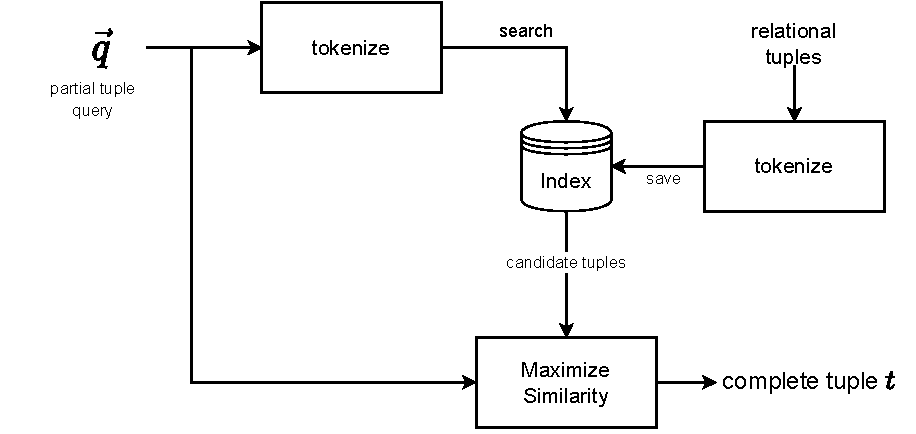
\includegraphics[width=0.8\textwidth]{my/graphics/tuple_completion.pdf}
	\caption{Matching a partial tuple $\vec{q}$ to a complete tuple $t$}
	\label{fig:tuple_completion}
\end{figure}

We use a neural network to optimize the query processing pipeline. Detailed description can be found in  Section~\ref{sec:opt_pipeline}. We define the neural network classifier as:

\begin{definition}[Neural network classifier]
%	what is the input to the neural network, and what you are learning?
	Let $R_1, R_2, R_3, \dots, R_K$ be $K$ relations. The neural network classifier takes a partial tuple query $\vec q$ and estimates the probabilities that the search result of $\vec q$ belongs to relation $R_i$, $\forall i \in \{1, 2, \dots, K\}$.
	%Let $\mathbf{index}_1$, $\mathbf{index}_2$, $\dots$, $\mathbf{index}_K$ be $K$ full-text indexes corresponding to the $K$ relations.

 
%	Given a set of $N$ training examples $\mathbb X = \{(x^{(i)}, l^{(i)}): i = 1, 2, \dots, N\}$, where  $x^{(i)}$ is a (partial) tuple that belongs to $R_{l^{(i)}}$ ($l^{(i)} \in \{1, 2, ..., K\}$),
%	the goal is to train a neural network classifier that takes a partial tuple query $\vec q$ and estimates the probabilities that the search result of $\vec q$ belongs to relation $R_i$, $\forall i \in \{1, 2, \dots, K\}$.
\end{definition}

%	Note that we use full-text index to support partial tuple search, and we partition full-text index to mitigate the impact of bottleneck casued by hashing collision in inverted term index data structure. More details about partitioning of full-text index are given in Section~\ref{subsection:partition_text_index}.

\section{Partial tuple search using full-text search}
\label{sec:search_fulltext_index}
Traditional full-text indexes, such as Apache Lucene, support keyword queries over large document collections using an inverted index data structure.  In this section, we describe how a full-text index is incorporated as the first stage of the query processing pipeline for partial tuple search.

The advantages of using a full-text index are:

\begin{itemize}
    \item Flexible and partial string matching between query keywords and document text
    \item Efficient query processing provided that the inverted document lists are not too long due to collisions.
\end{itemize}

We first encode complete relational tuples as documents to be stored in the full-text index.
The partial tuple query $\vec q$ is encoded as a keyword query.  It is important to point out that we must specify
the same tokenizer to convert relational tuples and query tuples to tokenized terms.  We use the 3-gram tokenizer to support fuzzy string matching for the values.

The full-text index evaluates the keyword query, and computes a top-$k$ result set of the best matching documents as relational tuple candidates.  These top-$k$ candidates guarantee high similarity between the labeled values in $\vec q$ and those in relational tuples.

\subsection{Encoding of tuples as documents}

Let us denote the tokenizer function as $\Tokenize$. A tuple $\vec r$ is converted into a document $\mathrm{doc}$ as follows:

$$
\Attr(\mathrm{doc}) = \Attr(\vec r) \cup \{\mathtt{fulltext}\}
$$
For each $a\in\Attr(\vec r)$,
$$
\mathrm{doc}[a] = \Tokenize(\vec r[a])
$$
Also,
$$
\mathrm{doc}[\mathtt{fulltext}] =\bigcup\big\{\Tokenize(\vec r[a]): a\in\Attr(\vec r)\big\}
$$
The special field $\mathtt{fulltext}$ of $\mathrm{doc}$ contains all tokenized terms of the tuple $\vec r$.

\begin{example}
Given a tuple $\vec r$ as:
$$
(\mathrm{Name}:Jack,\ \mathrm{Address}:100\ Simcoe\ Street)
$$
Its attributes $\Attr(\vec r)$ are $\{\mathrm{Name}, \mathrm{Address}\}$. Therefore, the document attributes  $\Attr(doc)$ are $\{\mathrm{Name},\ \mathrm{Address},\ \mathrm{fulltext}\}$.

If we use a standard tokenizer, the result of tokenization will be,
$$
\left[\begin{array}{rcl}
\mathrm{Name} & \mapsto & \makebox{Jack} \\
\mathrm{Address} & \mapsto & \makebox{100, Simcoe, Street} \\
\mathrm{fulltext} & \mapsto & \makebox{Jack, 100, Simcoe, Street}
\end{array}\right]
$$

On the other hand, if we use a character-based 3-gram tokenizer with a special padding character ``\_", the result will be,
$$
\left[\begin{array}{rcl}
\mathrm{Name} & \mapsto & \makebox{\_\_J \_Ja Jac ack ck\_ k\_\_} \\
\mathrm{Address} & \mapsto & \makebox{\_\_1 \_10 100 00\_ 0\_\_ \_\_S \_Si Sim imc mco coe oe\_ e\_\_ \_\_S \_St Str tre ree eet et\_ t\_\_} \\
\mathrm{fulltext} & \mapsto & \makebox{\_\_J \_Ja Jac ack ck\_ k\_\_ \_\_1 \_10 100 00\_ 0\_\_ \_\_S \_Si Sim imc mco coe oe\_ e\_\_ \_\_S} \\ 
 & & \makebox{\_St Str tre ree eet et\_ t\_\_}\\
\end{array}\right]
$$

\end{example}

\subsection{Encoding partial tuple queries as keyword queries}

Given a partial tuple $\vec q$, we want to encode it as a keyword query such that the search engine can
find the documents that correspond to the relevant tuples.

For each labeled value $(l_i, x_i)$ in the partial tuple, we generate a query clause.

\begin{itemize}
\item If $l_i\not= ?$, then the query clause is $q_i = l_i:x_i$.
\item If $l_i = ?$, then the query clause is $q_i = \mathtt{fulltext}:x_i$.
\end{itemize}

The generated query is:
$$ q = q_1\ \mathbf{or}\ q_2\ \mathbf{or}\ \dots $$

One can see that any complete tuple $\vec r$ that satisfy the query $\vec q$ will have its encoding document satisfying the keyword query $q$.

\subsection{From search results to partial tuple completion}

For our problem, we need to match the partial tuple $\vec q$ with a complete tuple $t$.  This can be done
by further post-process the documents in search results returned by the search engine. 

%Recall that a tuple matching is a function $h: \mathrm{LV}(t) \to \mathrm{LV}(\vec q)$.  
Recall that a tuple matching is a function $h: \mathrm{LV}(\vec q) \to \mathrm{LV}(t)$, where $\mathrm{LV}(\vec q)$ and $\mathrm{LV}(t)$ are labeled values of $\vec q$ and $t$, respectively.
The top completion of $\vec q$ should be a complete tuple that has the highest matching score based on the similarity measure.  Since the search engine already returns the top-$k$ candidate documents, we can compute the optimal matching
between $\vec q$ to each of the candidates in order to rank the candidates with respect to their matching scores.

Finding optimal matching of labeled values from the partial tuple $\vec q$ to  a candidate tuple $t$ is equivalent to solving the maximum weighted matching of a bipartite graph.

Define the graph $G$ as:
\begin{itemize}
    \item The vertices are: $V = \mathrm{LV}(t)\cup\mathrm{LV}(\vec q)$.
    \item The edges and their respective weights are defined as:
        $$E = \{\left<x_1, x_2, \Sim(V(x_1),V(x_2)\right>: x_1\in\mathrm{LV}(t)\makebox{ and }
        x_2\in\mathrm{LV}(\vec q)
        \makebox{ and } (L(x_1)=L(x_2) \makebox{ or } L(x_2)=?)\}$$ 
       where $L(x_1)$ and $L(x_2)$ are labels of $x_1$ and $x_2$, respectively.
    \item $G$ is the weighted graph $(V, E)$.
\end{itemize}

%The max-weighted matching of $G$ is necessarily a matching $h$ from $\mathrm{LV}(t)$ to $\mathrm{LV}(\vec q)$.
The max-weighted matching of $G$ is necessarily a matching $h$ from $\mathrm{LV}(\vec q)$ to $\mathrm{LV}(t)$.
The weight sum of $h$ is the matching score based on the similarity of matched labeled values.  It is now that the optimal matching can be
found exactly in polynomial time using various algorithms, e.g., Hungarian algorithm \cite{cormen2022introduction}.



\section{Optimizing query processing pipeline with neural networks}
\label{sec:opt_pipeline}

As described in Section~\ref{sec:fuzzy-collision}, a potential bottleneck associated with inverted index structures for full-text search is the hashing collision which creates long linked lists
at the leaf nodes of the index tree (See Figure~\ref{fig:inverted_term_index}).

In our application, the character based 3-gram tokenizer will generate a compact vocabulary consisting
of at most $|\mathrm{charset}|^3$ distinct tokens where $\mathrm{charset}$ is the total character set.  So, when the number of documents grow greater than $|\mathrm{charset}|^3$, the linked lists at the leaf nodes will grow linearly with respect to the number of relational tuples.

The concern is that the full-text index will degrade as the dataset size grows due to the 3-gram tokenization that we employ to support fuzzy string matching.  Unfortunately, our experimental evaluation in Section~\ref{subsection:perf_baseline_expt} confirms the performance degradation in practice.

In this section, we will describe a method to perform partitioning of the full-text index to overcome the performance bottleneck caused by hash collisions.

Our method utilizes a neural network to optimize the index access order during partial tuple search.  The neural network is to be embedded in the overall query processing pipeline, and will be self-supervised based on existing data.

\subsection{Partition of full-text index}
\label{subsection:partition_text_index}
An aggregated index is a function as follows:
$$\mathbf{index} : \mathbf{Query} \to \mathbf{List}[\mathbf{Tuple}]$$
It indexes all the tuples from every relation.

However, we advocate to partition the tuples based on the relation they below to.  Thus,
if we have relations $R_1, R_2, R_3, \dots, R_n$, we will have $n$ indexes
$\{\mathbf{index}_1$, $\mathbf{index}_2$, $\dots$, $\mathbf{index}_n\}$, each indexing the tuples
of a single relation.

$$\mathbf{index}_i : \mathbf{Query} \to \mathbf{List}[\mathbf{Tuple}]$$

The search can be done concurrently over all indexes:

\begin{verbatim}
priority_queue
for index_i in all_indexes {
  spawn index_i.search(q) into priority_queue
}
\end{verbatim}

We can also do sequential access of the indexes:

\begin{verbatim}
for index_i in sorted(all_indexes, q) {
    index_i.search(q) into priority_queue
}
\end{verbatim}

In this thesis we focus on the sequential access approach in favour of saving CPU load.
The challenge is to sort the indexes dynamically based on the user query $\vec q$.
The sorting should place relations that can satisfy $\vec q$ with higher priority, so that
successful matches are found as early as possible.

Thus, our strategy to sort the indexes is based on a sorting key function:
$$
S : (\mathbf{index}_i, \vec q) \to [0, 1] \mapsto \mathbf{prob}(\mathrm{result}(\vec q) \in R_i)
$$

The sorting score $S(\mathbf{index}_i, \vec q)$ is the (estimate of the) probability that the search
result of $\vec q$ belongs to the relation $R_i$.  Since there are only a finite many relations,
we can reformulate the scoring function $S$ to as an $n$-way classification function:

$$
\mathbf{classify} : \vec q \mapsto \left[
\begin{array}{c}
    S(\mathbf{index}_1, \vec q) \\
    S(\mathbf{index}_2, \vec q) \\
    \vdots \\
    S(\mathbf{index}_n, \vec q)
\end{array}
\right]
$$

Our objective is to learn the $\mathbf{classify}$ function using a neural network.

\subsection{Vectorization of queries}

The classifier can be trained using a neural network that can be embedded in the query processing pipeline.
The design objectives are:
\begin{itemize}
    \item The neural network must be compact in size so that it incurs minimal performance overhead, and can be embedded in a search system.
    \item The training of the network must require minimal manual intervention.  Thus the neural network must be trained with self-supervision from existing data.
\end{itemize}

The classification function is:

\begin{equation}
    \mathbf{classify} : \mathbf{Query} \to \mathbb{R}^n
\end{equation}
where the output of $\mathbf{classify}$ is the probability distribution over the $n$ partitioned indexes. Elements we presented in Section~\ref{sec:neural-networks} present several options for the neural network architecture.

\noindent{\bf Token representation of queries}:  given a query $\vec q=\{(l_i, x_i): 1\leq i \leq m\}$, we generate the text representation of the query by simply concatenating the text representation of labels and the tokenized query values.

$$
\mathbf{tokens}(\vec q) = \{l_1\} \oplus \mathbf{tokenize}(x_1) \oplus \{l_2\} \oplus \mathbf{tokenize}(x_2) \oplus \dots
\{l_m\} \cup \mathbf{tokenize}(x_m)
$$
where $\oplus$ is sequence concatenation.

\noindent{\bf Integer encoding of queries}: next we encode $\mathbf{tokens}(\vec q)$ using a universal
vocabulary $\mathbf{vocab}$.  The vocabulary consists of all known tokens, and their respective
ordinal integer code.  This vocabulary will be built using the existing relational tuples.  The construction of the vocabulary is described in subsequent sections.  The vocabulary is described as a function from tokens to integers:
$$ \mathbf{vocab} : \mathbf{Token} \to \mathbb{N}$$

The integer sequence of a query is given by:
$$
\mathbf{sequence}(\vec q) = \mathbf{vocab}\circ\mathbf{tokens} (\vec q) \in\mathbb{N}^*
$$

\noindent{\bf Embedding vectors of queries}:
Using a standard embedding layer (Section~\ref{sec:embedding-layer}), embed the integer sequence representation of the query
to a sequence of latent vectors.

$$
\mathbf{vector}(\vec q) = \mathbf{Embedding}(\mathbf{sequence}(\vec q))\in\mathbb{R}^{|q|\times d}
$$

At this point, we have many options in mapping
the vector sequence to the probability distribution
in $\mathbb{R}^n$.

For the remainder of this chapter, we denote the vector sequence representation of $\vec q$ as:

$$\vec x = \mathbf{sequence}(\vec q) = (x_1, x_2, \dots, x_{|q|})$$
where each $x_i\in\mathbb{R}^d$ is the embedding vector 
of the $i$-th token in a $d$-dimensional latent space.

\subsection{Neural network architectures for query classification}
\label{sec:architectures}

\noindent{\bf MLP based classification}.

Given the input of vectorized query representation $\vec x$, 
we first flatten it using global average over the entire sequence length.  Then, we process it with a MLP with softmax
activation function.  The MLP must have $n$ output neurons.

$$
\begin{array}{rlr}
&\vec x  & (|q|, d) \\
\to & \left(\frac{\sum_{i=1}^{|q|} x_i}{|q|}\right) & (d) \\
\to & \mathbf{MLP}(\makebox{output-dim}=n) & (n) \\
\to & \mathbf{softmax}(\cdot) & (n) \\
\end{array}
$$

\noindent{\bf Recurrent network architecture with LSTM cells}.

Since recurrent neural networks (RNN) are specifically designed to process sequence inputs, we can utilize
a RNN to map the input $\vec x$ to a flattened state vector, which can then be processed
by a MLP to compute the output probability distribution.

The advantage of RNN is that it can learn inter-token dependencies in the query at the cost of
a bigger model size and higher training cost.

$$
\begin{array}{rlr}
&\vec x  & (|q|, d) \\
\to & \mathbf{LSTM}(\makebox{output-state=True}) & (d) \\
\to & \mathbf{MLP}(\makebox{output-dim}=n) & (n) \\
\to & \mathbf{softmax}(\cdot) & (n) \\
\end{array}
$$

\noindent{\bf 1D convolution architecture}.

Another standard technique to learn sequential features is to use 1D convolution.
The 1D convolution layer (Section~\ref{sec:cnn}) produces a sequence of {\em feature} vectors
that capture the short-range token dependencies within the convolution window size.  We then use
global averaging to flatten the convolution features for further processing using a MLP.

$$
\begin{array}{rlr}
&\vec x  & (|q|, d) \\
\to & \mathbf{Conv1D} & (|q|, d) \\
\to & \mathbf{Global\ Average} & (d)\\
\to & \mathbf{MLP}(\makebox{output-dim}=n) & (n) \\
\to & \mathbf{softmax}(\cdot) & (n) \\
\end{array}
$$

\noindent{\bf Transformer and MLP Mixer}

Transformers have shown to be a superior architecture for many tasks in the domain of MLP and sequence learning.  The exact architecture of a transformer block is shown in the implementation section (See Figure~\ref{fig:transformer_model}).  Due to the nature of our problem, we chose to use only a single transformer block so that the model remains small enough to be embedded in the query processing pipeline.

A more recent MLP based architecture is MLP mixer which is a concatenation of two MLP layers separated by a matrix transpose operation.  Details of the MLP mixer are shown in Figure~\ref{fig:mlpmixer_model}.

\subsection{Unsupervised training of neural network classifiers}

The classifier needs to be trained with data of the following form:
$$
(\vec q, i)
$$
where $\vec q$ is a sample query, and $i$ is the relation $R_i$ that contains the best matching
tuple of $\vec q$.

The training data is generated directly from the relational tuples from the database.  For each complete tuple $\vec r = \{(l_i, x_i): i\in I\}$, we formed a query $\vec q_r$ by random sampling from
the labeled values while masking the labels.

$$
\vec q_r = \{(?, x_i): i\in\mathbf{sample}(I)\}
$$

Thus, given a database with $n$ relations $R_1, R_2, \dots, R_n$:
$$
\mathbf{train} = \bigcup_{i=1}^n\{(\vec q_r, i): r\in R_i\}
$$

\section{Overall query processing pipeline}

To summarize the proposed query processing pipeline for partial tuple search, we have the following stages:

\begin{enumerate}
    \item A partial tuple is entered as user input.
    \item The partial tuple is tokenized and converted to a structured keyword query.
    \item The neural network classifier sorts the partitioned indexes based on the probability scores.
    \item The partitioned indexes are scanned to find top-$k$ complete tuple candidates from the database.
    \item The candidates are ranked by max-matching based similarity scores.
\end{enumerate}

Our pipeline requires that partitioned full-text indexes are built from tuples of each relation in offline mode. In addition, the neural network classifier should be trained using sampled tuples from each relation.

In Chapter~\ref{ch:implementation-evaluation}, we will describe the implementation of each neural network architecture. We will also discuss the experimental evaluation and comparison of the performance gain of each neural network architecture.
\chapter{Implementation and Performance Evaluation of Neural Networks For Index Acceleration}
\label{ch:implementation-evaluation}

In the previous chapter, we have presented the neural network based algorithm to accelerate the partial tuple search of relational data.  Our algorithm relies on a partial tuple classifier to optimize the ordering of text index search.  In particular, we have shown that a variety of neural network architectures can be used in the design of the classifier.

In this chapter, we will describe the evaluation of the proposed solutions.  We will verify the effectiveness and limitations of our solutions, and perform a comparative study of different network architectures.  For each network architecture, we will present the benefits and drawbacks, and provide our understanding of the explanation of the observations.

\section{Some assumptions about datasets}
\label{sec:assumption}
In this section, we list some assumptions for our experimental evaluation:
\begin{itemize}
	\item The numbers of tuples of relations are not skewed, this is, there is no relation that has an extremely large number of tuples than other relations.
	\item Applying operations of inserting new tuples, updating or deleting existing tuples to a database does not introduce new vocabulary.
\end{itemize}

These assumptions imply limitations of our proposed solutions. We will provide some discussion about the limitations and possible future work in Section~\ref{sec:limitation}.

\section{Datasets}
The datasets we have used to evaluate our system is a collection of survey data from Statistics Canada \cite{ds01, ds02, ds03, ds04, ds05, ds06, ds07, ds08, ds09, ds10}, which includes one labour force survey, six COVID-19 surveys, one income survey, one community health survey, and one housing survey.
They offer many real-world characteristics that pose as challenges to  neural network classifiers.  Given the intended application scenarios of our research, we felt that it was important to evaluate our work using real-world datasets. For easy reference in subsequent sections, we give each dataset an id, as shown in Table \ref{table:id_name}.   
\begin{table}[t]
	\centering
	\begin{tabularx}{\textwidth}{|l|X|}
		\hline
		\textbf{Dataset id} & \textbf{Dataset name} \\
		\hline
		ds01 & Labour Force Survey, April 2019 [Canada] \\
		ds02 & Crowdsourcing: Impacts of COVID-19 on Canadians’ Experiences of Discrimination Public Use Microdata File \\
		ds03 & Crowdsourcing: Impacts of COVID-19 on Canadians Public Use Microdata File, [2020] \\
		ds04 & Crowdsourcing: Impacts of the COVID-19 on Canadians – Your Mental Health Public Use Microdata File, [2020] \\
		ds05 & Crowdsourcing: Impacts of COVID-19 on Canadians' Perception of Safety Public Use Microdata File, [2020] \\
		ds06 & Crowdsourcing: Impacts of the COVID-19 on Canadians – Trust in Others Public Use Microdata File [2020] \\
		ds07 & Impacts of the COVID-19 pandemic on postsecondary students (ICPPS) 2020, Crowdsource file, Public use microdata file \\
		ds08 & Canadian Income Survey (CIS), 2017 \\
		ds09 & Canadian Community Health Survey - Annual Component (CCHS) 2017-2018 \\
		ds10 & Canadian Housing Survey, 2018 \\
		\hline
	\end{tabularx}
	\caption{Dataset ids and names}
	\label{table:id_name}
\end{table}

These 10 datasets contain both numerical and textual data with different numbers of attributes and tuples. For example, the labour force survey contains data of the Canadian labour market. It has total 60 attributes related to the job market, such as employment status, industry, status of working full-time or part-time, hourly wage, etc. Table \ref{tab:ds01_samples} shows 5 samples with a subset of 10 attributes. The descriptions of the selected 10 attributes are shown in table \ref{tab:ds01_attrs_samples}.
\begin{table}[!ht]
	\centering
	\resizebox{\textwidth}{!}{%
		\begin{tabular}{
				|c
				|c
				|>{\raggedright\arraybackslash}p{0.1\textwidth}
				|>{\raggedright\arraybackslash}p{0.1\textwidth}
				|l
				|>{\raggedright\arraybackslash}p{0.2\textwidth}
				|>{\raggedright\arraybackslash}p{0.2\textwidth}
				|>{\raggedright\arraybackslash}p{0.2\textwidth}
				|l
				|l|}    \hline
			\multicolumn{1}{|c|}{\textbf{survyear}} &
			\multicolumn{1}{c|}{\textbf{survmnth}} &
			\multicolumn{1}{c|}{\textbf{lfsstat}} &
			\multicolumn{1}{c|}{\textbf{prov}} &
			\multicolumn{1}{c|}{\textbf{age\_12}} &
			\multicolumn{1}{c|}{\textbf{educ}} &
			\multicolumn{1}{c|}{\textbf{immig}} &
			\multicolumn{1}{c|}{\textbf{noc\_10}} &
			\multicolumn{1}{c|}{\textbf{ftptmain}} &
			\multicolumn{1}{c|}{\textbf{hrlyearn}} \\ \hline
			2019 &
			April &
			Employed, at work &
			Ontario &
			25 to 29 years &
			Postsecondary certificate or diploma &
			Non-immigrant &
			Natural resources, agriculture and related production occupations &
			Full-time &
			33.00 \\
			2019 &
			April &
			Not in labour force &
			British Columbia &
			70 and over &
			Bachelor\Verb|''|s degree &
			Non-immigrant &
			&
			&
			\\
			2019 &
			April &
			Employed, at work &
			British Columbia &
			45 to 49 years &
			High school graduate &
			Non-immigrant &
			Business, finance and administration occupations &
			Full-time &
			26.00 \\
			2019 &
			April &
			Employed, at work &
			Ontario &
			20 to 24 years &
			Postsecondary certificate or diploma &
			Non-immigrant &
			Health occupations &
			Full-time &
			37.60 \\
			2019 &
			April &
			Employed, at work &
			Ontario &
			70 and over &
			Some postsecondary &
			Immigrant, landed more than 10 years earlier &
			Occupations in art, culture, recreation and sport &
			Part-time &
			32.00 \\ \hline
		\end{tabular}%
	}
	\caption{5 samples from the labour force survey dataset ``ds01", showing only 10 attributes.}
	\label{tab:ds01_samples}
\end{table}
\begin{table}[t]
	\centering
	\begin{tabular}{|l|l|}
		\hline
		\multicolumn{1}{|c|}{\textbf{Attribute}} & \multicolumn{1}{c|}{\textbf{Description}}     \\ \hline
		survyear & Survey year                        \\
		survmnth & Survey month                       \\
		lfsstat  & Labour force status                \\
		prov     & Province                           \\
		age\_12  & Five-year age group of respondent  \\
		educ     & Highest educational attainment     \\
		immig    & Immigration status                 \\
		noc\_10  & 2016 NOC (10 categories)           \\
		ftptmain                                 & Full- or part-time status at main or only job \\
		hrlyearn & Usual hourly wages, employees only \\ \hline
	\end{tabular}
	\caption{10 attributes and their descriptions from the labour force survey dataset ``ds01".}
	\label{tab:ds01_attrs_samples}
\end{table}
Table \ref{table:ds_stats} shows the number of attributes and tuples in each dataset.
\begin{table}[t]
	\centering
	\begin{tabular}{ |l|r|r|r|r|r|r|r|r|r|r| }
		\hline
		\textbf{Dataset id} & \textbf{No. of attrs.} & \textbf{No. of tuples} \\
		\hline
		ds01 & 60 & 100,885 \\
		ds02 & 129 & 36,662 \\
		ds03 & 47 & 242,512 \\
		ds04 & 43 & 45,989 \\
		ds05 & 23 & 43,631 \\
		ds06 & 47 & 36,538 \\
		ds07 & 42 & 101,902 \\
		ds08 & 194 & 92,286 \\
		ds09 & 1051 & 113,286 \\
		ds10 & 132 & 61,750 \\
		\hline
	\end{tabular}
	\caption{Number of attributes and tuples in each dataset.}
	\label{table:ds_stats}
\end{table}

Sometimes different datasets share common attributes. For example, the COVID-19 datasets have a common attribute about community size and metropolitan influence zones where the survey correspondents live in. By using multiple partial tuple completion, users can ``jump" from one dataset to another. For example, users may find some data related to discrimination from the dataset of impacts of COVID-19 on Canadians’ experiences of discrimination. Then they can use the results to search more information about people's perception of safety in the communities with the same sizes in the dataset of impacts of COVID-19 on Canadians’ perception of safety. This will help users to gain more insights from the survey results.

\section{Architecture and software stack}
In order to thoroughly evaluate the end-to-end search system, we have developed a platform with the following technology stack.  We use Lucene \cite{lucene} as the full-text index.  A customized search engine is developed on top of Lucene to support partial tuple search queries.  This is necessary for us to have detailed instrumentation to collect performance metrics, and to gain control over the ordering of text index search.  We have implemented all neural network based classifiers using TensorFlow \cite{tensorflow}. The trained models are used to generate the ordering of Lucene index access. 
The evaluation of the neural network acceleration is based on the speed-up of query performance between the machine learning generated ordering and other alternatives.
In addition, top-$k$ accuracy is also used to evaluate models.
The query workloads used in evaluation are generated from the datasets themselves. Figure \ref{fig:proj_arch} shows the high-level architectural overview of our implementation. More details about the training datasets and the query workload generation will be presented in subsequent sections.
\begin{figure}[!th]
	\centering
%	\includesvg[inkscapelatex=false, width = 250pt]{overall_architecture.svg}
	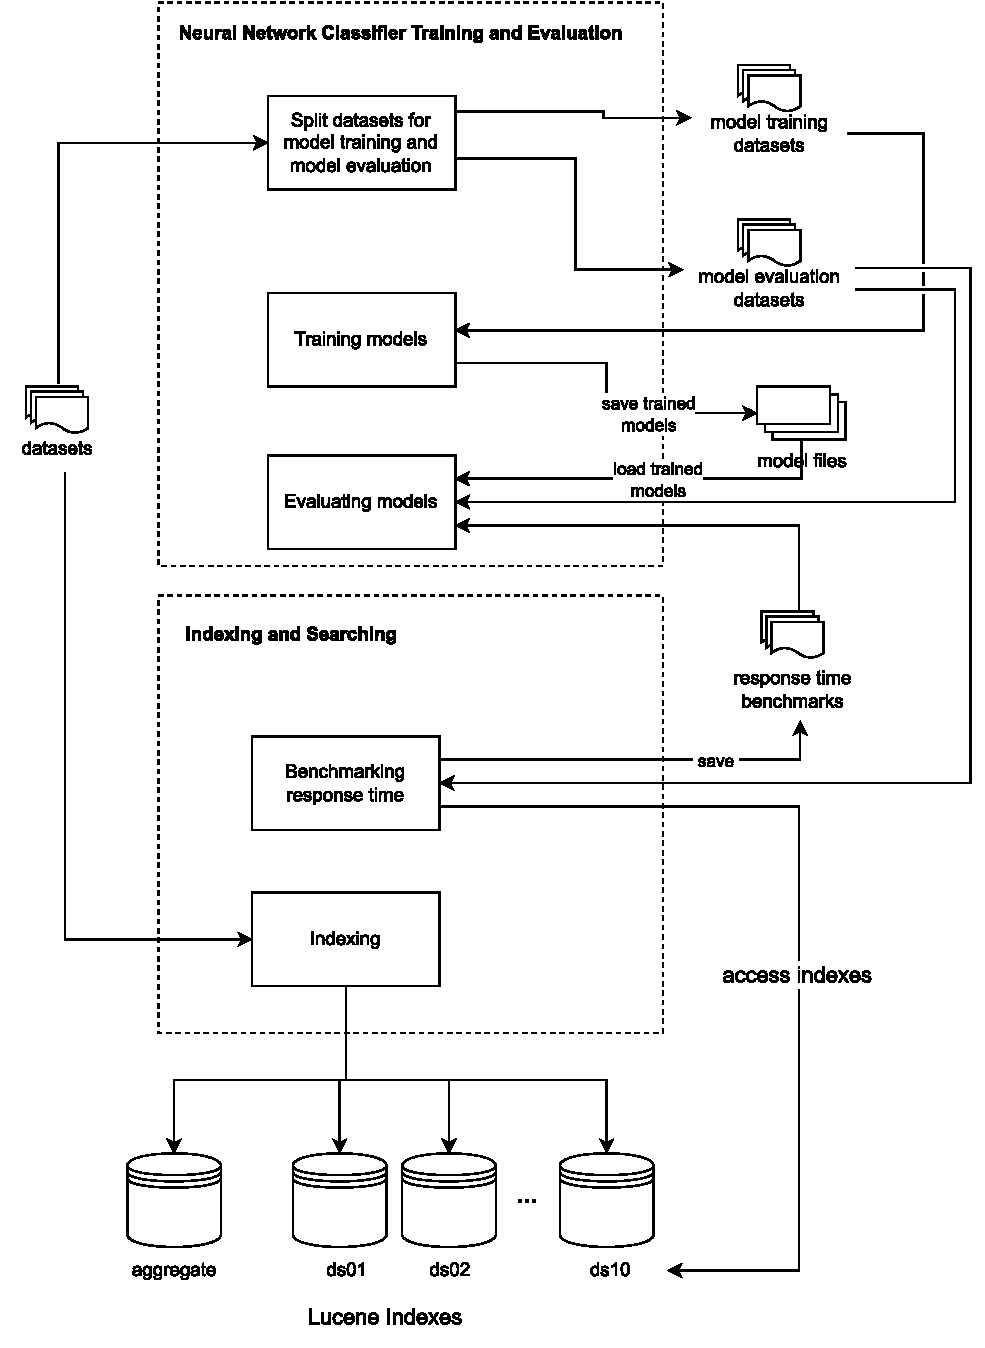
\includegraphics[width=0.8\textwidth]{my/graphics/overall_architecture.pdf}
	\caption{High-level overview of architecture}
	\label{fig:proj_arch}
\end{figure}

\subsection{Lucene and a customized search engine}
We developed a customized search engine on top of Lucene. It has two main functions. The first is to index datasets to create Lucene indexes. 
When indexing datasets, each tuple is converted to a Lucene document, which contains a set of \emph{(attribute name, attribute value)} pairs. We apply character-based 3-gram tokenization to attribute values. We use the special character ``\_" for padding. In addition, we add an extra field ``fulltext" to the document, which contains all 3-gram tokens of all attribute values. This field is needed to support full-text search.
For example, given a tuple $t$ as, 
$$
\{\mathrm{Name}:Jack,\ \mathrm{Gender}:Male,\ \mathrm{Occupation}:\makebox{Software developer}\}
$$
our search engine will first apply Lucene's standard tokenization, and then our character-based 3-gram tokenization. The resulting Lucene document will be,
$$
\left[\begin{array}{rl}
\mathrm{name}: & \_\_j\ \_ja\ jac\ ack\ ck\_\ k\_\_ \\
\mathrm{gender}: & \_\_m\ \_ma\ mal\ ale\ le\_\ e\_\_ \\
\mathrm{occupation}: & \_\_s\ \_so\ sof\ oft\ ftw\ twa\ war\ are\ re\_\ e\_\_\ \_\_d\ \_de\ dev\ eve\ vel \\
& elo\ lop\ ope\ per\ er\_\ r\_\_ \\
\mathrm{fulltext}: & \_\_j\ \_ja\ jac\ ack\ ck\_\ k\_\_\ \_\_m\ \_ma\ mal\ ale\ le\_\ e\_\_\ \_\_s\ \_so\ sof \\
& oft\ ftw\ twa\ war\ are\ re\_\ e\_\_\ \_\_d\ \_de\ dev\ eve\ vel\ elo\ lop\ ope \\
& per\ er\_\ r\_\_
\end{array}\right]
$$

The second main function is to support partial tuple search queries. We also use character-based 3-gram tokenization when constructing a search query. For example, given a partial tuple as:
$$
\{\mathrm{Name}:Jack,\ \mathrm{Gender}:Male\}
$$
the search query will be:
$$
\{\mathrm{fulltext}: \_\_j\ \_ja\ jac\ ack\ ck\_\ k\_\_\ \_\_m\ \_ma\ mal\ ale\ le\_\ e\_\_\}
$$

\subsection{Partitioned indexes and an aggregate index}

We have indexed the tuples from all datasets into a single Lucene index.  The tuples are tokenized  using the 3-gram tokenizer in order to support fuzzy string matching as described in Section~\ref{sec:fuzzy-collision}.  This index will be referred to as the {\em aggregate index} since it contains all the tuples from 10 datasets in a single index.  The aggregate index contains approximately 877,000 documents.

We also have an alternative way of indexing the tuples using Lucene.  We partition the tuples based on which relation they belong to.  Given that we have 10 datasets, we have created 10 individual indexes, each containing the tuples from their respective relation.  We refer to the set of indexes as {\em partitioned indexes}.
The number of documents in each partitioned index is the same as the number of tuples in each dataset, as shown in Table \ref{table:ds_stats}.

With the two types of indexing schemes (partitioned vs aggregate indexing), we have many alternatives in evaluating a user query.

\noindent {\bf Aggregate index lookup:} we can simply issue the user query against the aggregate index as it contains all the available tuples.  

\begin{itemize}
    \item Pro: This is the traditional approach. It requires the least system design. Only a single thread is needed for each user query.
    \item Con: As we have indicated previously and will show in our experimental evaluation, this approach suffers from a performance bottleneck resulting from high token hashing collision rate.
\end{itemize}

\noindent {\bf Parallel lookup of partitioned indexes:} we can issue the query against all individual index in the partitioned index set.  This will perform parallel index lookup using multiple concurrent threads.

\begin{itemize}
    \item Pro: The result can be found quickly.  The index with the {\em correct} tuple will contain much less documents compared to the aggregate index, and thus will respond with the search result faster.  In fact, we argue that this is the optimal performance one can expect.
    \item Con: The concurrency will impose a higher CPU and disk IO demand as each user query will take up to $n$ threads to process.  In high traffic or low resource scenarios, this may be prohibitively expensive.
\end{itemize}

{\noindent \bf Predictive sequential lookup of partitioned indexes}: we advocate to perform single threaded  access of the partitioned indexes.  But rather than simple or random sequential scan of the index set, we utilize predictive neural networks to generate an optimized access pattern, as described in Section~\ref{sec:opt_pipeline}.

\begin{itemize}
    \item Pro: This method enjoys the advantage of both single-threaded index lookup and  low disk latency due to the potential early hit in a smaller partitioned index.  So we argue that the predictive lookup will yield high query performance and low resource usage.
    \item Con: This method requires a self-supervised neural network to perform the prediction.
\end{itemize}

\section{Evaluation methodology}
We evaluate five model architectures, including Multilayer Perceptron (MLP), Long Short-Term Memory (LSTM), 1D Convolution (Conv1D), Transformer and MLP-Mixer. We also exam how misspelled keywords affect the models' top-5 accuracies.

We use two metrics for model evaluation. The first metric is query processing time. We submit queries to partitioned indexes and the aggregate index, and record the response times as evaluation benchmark. More details are given in the subsection \ref{subsection:perf_baseline_expt}.

The second metric is top-$k$ accuracy. A model's prediction gives us the ordering of Lucene index access. If the Lucene index that a query belongs to is among the top-$k$ of the model's prediction, we consider the prediction accurate. For example, for a query sampled from \verb|ds02|, if the predicted access ordering is 
\begin{verbatim}
idx_ds06, idx_ds10, idx_ds07, idx_ds05, idx_ds02, ...
\end{verbatim}
we consider it an accurate top-5 prediction.

In the following subsections, we give more details about our training data, query workloads and experiments. We first describe how training data and query workloads are generated and tokenized in subsections \ref{subsection:training_data_gen} and \ref{subsection:query_workload_gen}, respectively. 
After that, we describe our experiments in subsections starting from  \ref{subsection:perf_baseline_expt} to  \ref{subsection:expt_3gram_resiliency}.

\subsection{Training data generation and tokenization}
\label{subsection:training_data_gen}
The raw datasets are in SAS7BDAT format, which is a binary database format. To make data processing easier for the downstream model training and evaluation, we convert all raw datasets to CSV files. Then we remove some unuseful attributes. For example, the labour force survey dataset contains the attribute \emph{rec\_num}, which indicates the record number in the file. This attribute is removed since it is not useful for our model training. After that the preprocessed CSV files are splitted into data for model training and data for model evaluation. Data for model evaluation are used to generate query workloads. More details about the query workloads generation will be presented in subsection \ref{subsection:query_workload_gen}.

Our next step is to generate training datasets from data reserved for model training. We randomly sample tuples from each CSV file without replacement. Then we normalize the sampled tuples to lowercase and remove special characters from them, which gives us word-based training data. In addition, we also apply character-based 3-gram tokenization to normalized tuples. We use ``\_" as the special character for padding in our implementation.  This results in 3-gram based training data. For example, given a raw tuple:
\begin{verbatim}
(2019,April,"Employed, at work",Nova Scotia,Other CMA or non-CMA,
45 to 49 years,,Female,Married,Above bachelor''s degree,
"Single jobholder")
\end{verbatim}
the normalized tuple will be:
\begin{verbatim}
(2019,april,employed at work,nova scotia,other cma or non cma,
45 to 49 years,female,married,above bachelors degree,
single jobholder)
\end{verbatim}
and the 3-gram tokenized tuple will be:
\begin{verbatim}
(__2 _20 201 019 19_ 9__,__a _ap apr pri ril il_ l__,__e _em emp mpl
plo loy oye yed ed_ d__ __a _at at_ t__ __w _wo wor ork rk_ k__,__n 
_no nov ova va_ a__ __s _sc sco cot oti tia ia_ a__,__o _ot oth the 
her er_ r__ __c _cm cma ma_ a__ __o _or or_ r__ __n _no non on_ n__ 
__c _cm cma ma_ a__,__4 _45 45_ 5__ __t _to to_ o__ __4 _49 49_ 9__ 
__y _ye yea ear ars rs_ s__,__f _fe fem ema mal ale le_ e__, __m _ma
mar arr rri rie ied ed_ d__,__a _ab abo bov ove ve_ e__ __b _ba bac
ach che hel elo lor ors rs_ s__ __d _de deg egr gre ree ee_ e__,__s
_si sin ing ngl gle le_ e__ __j _jo job obh bho hol old lde der er_
r__)
\end{verbatim}
Since we evaluate our models using partial tuple queries, a natural question is whether training models using partial tuples will have any impact on models' performance. Therefore, besides training datasets containing full tuples, we also create datasets containing partial tuples with 75\% and 50\% of attributes. Since each dataset will have an additional 3-gram tokenzed version, we have total six sets of training datasets. Table \ref{tab:training_vocab_size} shows their vocabulary sizes. In addition, we use dataset names as labels, so there is no need to manually label training tuples.
\begin{table}[t]
	\centering
	\resizebox{\textwidth}{!}{%
		\begin{tabular}{|l|ll|ll|ll|}
			\hline
			\multirow{2}{*}{\textbf{}} &
			\multicolumn{2}{c|}{\textbf{100\% attrs.}} &
			\multicolumn{2}{c|}{\textbf{75\% attrs.}} &
			\multicolumn{2}{c|}{\textbf{50\% attrs.}} \\ \cline{2-7} 
			&
			\multicolumn{1}{l|}{word-based} &
			3-gram based &
			\multicolumn{1}{l|}{word-based} &
			3-gram based &
			\multicolumn{1}{l|}{word-based} &
			3-gram based \\ \hline
			\multicolumn{1}{|c|}{vocabulary size} &
			\multicolumn{1}{r|}{56,482} &
			\multicolumn{1}{r|}{4,136} &
			\multicolumn{1}{r|}{47,536} &
			\multicolumn{1}{r|}{4,130} &
			\multicolumn{1}{r|}{37,183} &
			\multicolumn{1}{r|}{4,109} \\ \hline
		\end{tabular}%
	}
	\caption{Vocabulary size of six sets of training datasets.}
	\label{tab:training_vocab_size}
\end{table}

\subsection{Query workload generation and tokenization}
\label{subsection:query_workload_gen}
Query workloads are sets of partial tuples. 
We first randomly sample tuples from data reserved for model evaluation. 
Then we apply the same normalization process to them as we do to training datasets. 
After that we convert them to partial tuples by randomly sampling some attributes from them.
We create different workloads by varying the number of attributes sampled.
Table \ref{tab:workloads} shows two query workloads we used for model evaluation.
\begin{table}[t]
	\centering
	\begin{tabularx}{0.8\textwidth}{|l|X|}
		\hline
		\textbf{Workload name} & \textbf{Description} \\ \hline
		workload A & 5 randomly sampled attributes \\
		workload B & 3 randomly sampled attributes \\
		\hline
	\end{tabularx}
	\caption{Query workload names and descriptions.}
	\label{tab:workloads}
\end{table}

\subsubsection{Converting partial tuples to Lucene queries for searching}
We use Lucene's Query API to construct search queries from partial tuples. First we apply 3-gram tokenization to a partial tuple to get a list of tokens. Then we convert each token to a search term. After that we use the logical \verb|OR| operator to combine all search terms to form a query.
For example, given a partial tuple as the following:
\begin{verbatim}
no very easy no
\end{verbatim}
by adding the character ``\_" for padding, the constructed query will be:
\begin{verbatim}
__n OR _no OR no_ OR o__ OR __v OR _ve OR ver OR ery OR ry_ OR y__ OR
__e OR _ea OR eas OR asy OR sy_ OR y__ OR __n OR _no OR no_ OR o__
\end{verbatim}

\section{Experiments and observations}

In this section, we will enumerate over the experiments we conducted to evaluate our methodology.  For each experiment, we will focus on the motivation, experimental setup, the observation and their respective conclusions.

\subsection{Performance of aggregate vs optimal index lookup}
\label{subsection:perf_baseline_expt}
\noindent{\bf Description:}

Our first experiment tries to establish a baseline for the evaluation of our methodology using the query processing time. We measure three types of performance. The first is the optimal performance, which is achievable by parallel partitioned indexes lookup. The second is the performance of the aggregate index lookup. The last is the performance of sequential scan of all partitioned indexes. This will be the worst sequential scan if the predicted ordering of index access from our neural network classifiers puts the true partitioned index, i.e., the one contains the tuple, as the last one to scan.

To create the performance benchmark, we perform search against partitioned indexes and the aggregate index using the constructed partial tuple queries and log the response times. We repeat the process 10 times and compute the mean response times to be used as benchmark for model evaluation. Table \ref{tab:benchmark_A} and \ref{tab:benchmark_B} show the mean response times in milliseconds (ms) of the first 20 queries of the workload A and B, respectively. Both of the workloads have 1,000 queries. In both tables, the first 10 columns are the results of partitioned indexes, and the last one is that of the aggregate index. Details about the query workloads are described in subsection \ref{subsection:query_workload_gen}.
\begin{table}[!th]
	\centering
	\resizebox{\textwidth}{!}{%
		\begin{tabular}{|c|r|r|r|r|r|r|r|r|r|r|r|}
			\hline
			\textbf{} &
			\multicolumn{1}{c|}{\textbf{idx\_ds01}} &
			\multicolumn{1}{c|}{\textbf{idx\_ds02}} &
			\multicolumn{1}{c|}{\textbf{idx\_ds03}} &
			\multicolumn{1}{c|}{\textbf{idx\_ds04}} &
			\multicolumn{1}{c|}{\textbf{idx\_ds05}} &
			\multicolumn{1}{c|}{\textbf{idx\_ds06}} &
			\multicolumn{1}{c|}{\textbf{idx\_ds07}} &
			\multicolumn{1}{c|}{\textbf{idx\_ds08}} &
			\multicolumn{1}{c|}{\textbf{idx\_ds09}} &
			\multicolumn{1}{c|}{\textbf{idx\_ds10}} &
			\multicolumn{1}{c|}{\textbf{idx\_agg}} \\ \hline
			0  & 46.57   & 18.074  & 11.766 & 12.315 & 11.681 & 10.991 & 8.146   & 32.037 & 42.178  & 12.506 & 171.814 \\
			1  & 9.785   & 95.191  & 9.112  & 3.577  & 5.211  & 5.076  & 42.509  & 25.545 & 11.406  & 8.152  & 34.883  \\
			2  & 41.464  & 30.662  & 15.134 & 7.381  & 9.833  & 6.114  & 16.265  & 25.711 & 130.263 & 28.414 & 340.52  \\
			3  & 81.665  & 71.147  & 10.45  & 11.374 & 13.238 & 62.585 & 24.985  & 33.262 & 89.623  & 22.483 & 214.195 \\
			4  & 11.86   & 12.193  & 4.124  & 3.576  & 2.569  & 4.466  & 5.933   & 14.683 & 10.914  & 7.414  & 27.807  \\
			5  & 111.691 & 35.233  & 23.712 & 14.259 & 37.553 & 32.163 & 90.013  & 38.077 & 64.649  & 56.575 & 410.775 \\
			6  & 10.171  & 15.061  & 6.72   & 6.757  & 5.178  & 6.366  & 20.423  & 9.027  & 17.965  & 13.738 & 48.165  \\
			7  & 8.565   & 17.936  & 3.222  & 11.276 & 3.91   & 9.101  & 12.828  & 8.33   & 29.897  & 50.721 & 113.489 \\
			8  & 4.702   & 2.492   & 3.492  & 2.109  & 1.748  & 2.76   & 1.972   & 10.48  & 6.715   & 5.909  & 18.459  \\
			9  & 29.805  & 25.247  & 4.121  & 3.972  & 3.618  & 8.858  & 21.882  & 65.882 & 40.683  & 97.196 & 403.81  \\
			10 & 12.438  & 28.071  & 11.567 & 7.722  & 8.266  & 8.296  & 17.631  & 25.093 & 28.216  & 30.15  & 69.155  \\
			11 & 78.894  & 199.486 & 36.34  & 16.409 & 59.3   & 19.544 & 52.956  & 31.944 & 81.945  & 49.079 & 269.655 \\
			12 & 34.995  & 17.869  & 6.531  & 8.366  & 4.515  & 9.189  & 11.174  & 38.777 & 33.707  & 16.754 & 98.553  \\
			13 & 27.613  & 291.843 & 36.575 & 18.002 & 16.23  & 21.494 & 10.564  & 35.939 & 35.287  & 9.281  & 513.177 \\
			14 & 14.984  & 19.801  & 18.374 & 7.259  & 9.394  & 10.142 & 11.601  & 10.555 & 24.247  & 5.859  & 181.814 \\
			15 & 13.587  & 7.268   & 3.283  & 4.145  & 2.499  & 3.895  & 11.989  & 9.273  & 72.258  & 10.647 & 210.635 \\
			16 & 13.702  & 95.056  & 9.045  & 3.973  & 5.103  & 8.488  & 38.507  & 36.359 & 12.235  & 17.131 & 49.995  \\
			17 & 56.258  & 33.413  & 15.297 & 20.917 & 77.721 & 36.136 & 20.222  & 23.676 & 60.217  & 25.79  & 200.614 \\
			18 & 82.657  & 47.663  & 13.094 & 16.612 & 20.459 & 22.733 & 250.602 & 23.769 & 66.409  & 15.952 & 349.091 \\
			19 & 54.616  & 101.808 & 19.846 & 10.232 & 17.782 & 10.651 & 15.67   & 20.257 & 31.221  & 18.2   & 170.922 \\ \hline
		\end{tabular}%
	}
	\caption{Mean query processing time in milliseconds of the query workload A.}
	\label{tab:benchmark_A}
\end{table}
\begin{table}[!th]
	\centering
	\resizebox{\textwidth}{!}{%
		\begin{tabular}{|c|r|r|r|r|r|r|r|r|r|r|r|}
			\hline
			\textbf{} &
			\multicolumn{1}{c|}{\textbf{idx\_ds01}} &
			\multicolumn{1}{c|}{\textbf{idx\_ds02}} &
			\multicolumn{1}{c|}{\textbf{idx\_ds03}} &
			\multicolumn{1}{c|}{\textbf{idx\_ds04}} &
			\multicolumn{1}{c|}{\textbf{idx\_ds05}} &
			\multicolumn{1}{c|}{\textbf{idx\_ds06}} &
			\multicolumn{1}{c|}{\textbf{idx\_ds07}} &
			\multicolumn{1}{c|}{\textbf{idx\_ds08}} &
			\multicolumn{1}{c|}{\textbf{idx\_ds09}} &
			\multicolumn{1}{c|}{\textbf{idx\_ds10}} &
			\multicolumn{1}{c|}{\textbf{idx\_agg}} \\ \hline
			0  & 98.113 & 57.467  & 10.403 & 37.902 & 12.051 & 62.483 & 38.51   & 26.149 & 165.856 & 16.691  & 314.936 \\
			1  & 14.557 & 55.388  & 28.667 & 5.697  & 9.935  & 7.249  & 11.154  & 12.134 & 71.949  & 8.198   & 238.055 \\
			2  & 8.631  & 3.937   & 3.175  & 2.545  & 5.582  & 2.101  & 9.151   & 4.998  & 15.669  & 4.413   & 67.788  \\
			3  & 11.335 & 102.476 & 9.366  & 3.973  & 5.219  & 5.831  & 43.672  & 31.271 & 11.799  & 10.532  & 38.502  \\
			4  & 5.308  & 3.488   & 1.841  & 1.794  & 1.599  & 1.831  & 2.318   & 5.721  & 5.43    & 4.208   & 16.736  \\
			5  & 3.67   & 3.528   & 1.455  & 0.888  & 1.378  & 1.309  & 1.754   & 3.788  & 5.68    & 5.098   & 7.443   \\
			6  & 91.594 & 71.66   & 13.706 & 19.588 & 13.286 & 26.387 & 19.932  & 34.864 & 100.266 & 149.223 & 534.203 \\
			7  & 31.022 & 8.103   & 3.399  & 3.869  & 10.046 & 19.07  & 24.614  & 21.792 & 12.224  & 21.41   & 79.365  \\
			8  & 12.886 & 2.355   & 1.921  & 1.164  & 1.289  & 1.857  & 2.255   & 21.522 & 13.225  & 8.419   & 57.589  \\
			9  & 22.284 & 24.1    & 5.037  & 5.806  & 5.746  & 6.755  & 29.814  & 47.61  & 18.798  & 95.213  & 123.481 \\
			10 & 15.28  & 100.405 & 18.486 & 22.014 & 10.342 & 14.922 & 23.115  & 46.89  & 71.578  & 44.932  & 257.194 \\
			11 & 25.516 & 112.658 & 16.634 & 7.536  & 10.233 & 3.534  & 10.162  & 23.997 & 23.325  & 17.062  & 208.747 \\
			12 & 10.205 & 14.475  & 2.911  & 8.536  & 14.028 & 10.525 & 28.727  & 13.78  & 13.006  & 6.637   & 144.816 \\
			13 & 22.995 & 37.862  & 31.601 & 5.188  & 6.149  & 12.015 & 13.627  & 12.671 & 37.18   & 7.093   & 263.558 \\
			14 & 19.333 & 17.295  & 22.824 & 9.389  & 7.053  & 8.066  & 14.066  & 14.804 & 28.168  & 12.026  & 143.885 \\
			15 & 19.342 & 15.851  & 17.527 & 8.61   & 10.577 & 10.279 & 6.839   & 13.137 & 94.481  & 5.259   & 151.432 \\
			16 & 14.672 & 6.689   & 3.557  & 3.29   & 5.204  & 5.284  & 8.676   & 4.322  & 17.68   & 4.766   & 98.075  \\
			17 & 37.963 & 110.194 & 27.724 & 24.375 & 57.606 & 39.03  & 10.182  & 58.863 & 56.036  & 16.456  & 235.116 \\
			18 & 53.005 & 31.016  & 6.474  & 14.265 & 10.915 & 30.343 & 160.273 & 9.875  & 18.179  & 11.012  & 263.5   \\
			19 & 8.122  & 40.389  & 4.695  & 2.191  & 19.547 & 7.517  & 8.134   & 6.303  & 25.256  & 9.781   & 56.903  \\ \hline
		\end{tabular}%
	}
	\caption{Mean query processing time in milliseconds of the query workload B.}
	\label{tab:benchmark_B}
\end{table}

\noindent{\bf Observations:} 

As shown in figures \ref{fig:agg_vs_partitioned_A} and \ref{fig:agg_vs_partitioned_B}, the mean values of processing times of the worst sequential scan are longer than that of searching the aggregate index. The worst sequential scan is slower than searching the aggregate index by 45\% and 35\%, respectively. The goal of our neural network classifiers is to improve the performance of sequential scan by generating an optimized access pattern.
\begin{figure}[!th]
	\centering
	\begin{subfigure}{0.45\textwidth}
		\centering
		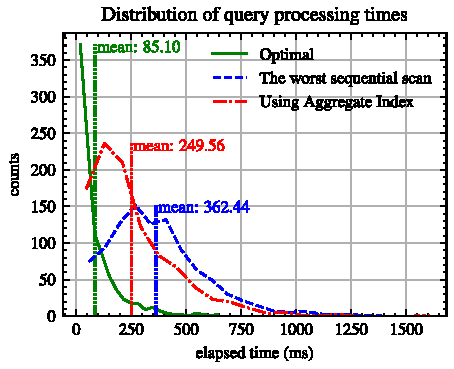
\includegraphics[]{my/graphics/agg_vs_partitioned_A.pdf}
		\caption{Workload A}
		\label{fig:agg_vs_partitioned_A}
	\end{subfigure}
	\hfill
	\begin{subfigure}{0.45\textwidth}
		\centering
		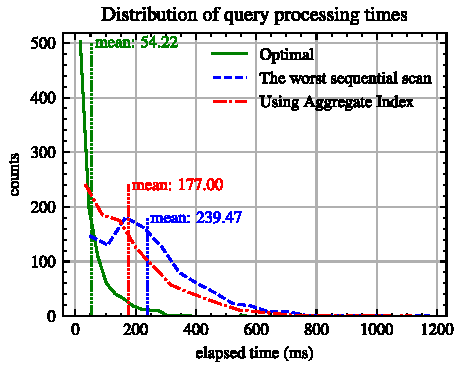
\includegraphics[]{my/graphics/agg_vs_partitioned_B.pdf}
		\caption{Workload B}
		\label{fig:agg_vs_partitioned_B}
	\end{subfigure}
	\caption{The distribution of query processing times of workload A and B.}
	\label{fig:agg_vs_partitioned_all}
\end{figure}

\subsection{Performance of optimal matching for partial tuple completion}
In this experiment, we examine the performance of optimal matching in three different steps.
In our first step, we set query size to be 10, tuple size to be 200, and edge connectivity density to be 0.1. We compute the optimal matching for 100 times and record the response times. Figure~\ref{fig:tuple_completion_1} shows the histogram of the results.
\begin{figure}[!th]
	\centering
	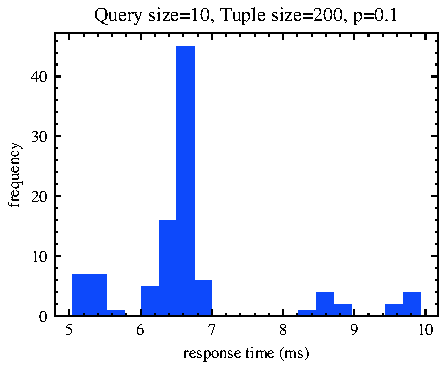
\includegraphics[width=0.6\textwidth]{my/graphics/tuple_completion_1.pdf}
	\caption{Distribution of optimal matching response times (ms)}
	\label{fig:tuple_completion_1}
\end{figure}
In our second step, we vary edge connectivity densities with the same fixed query size and tuple size as in step one. We repeat the process 100 times and compute the mean response times as results, which are shown in Figure~\ref{fig:tuple_completion_2}.
\begin{figure}[!th]
	\centering
	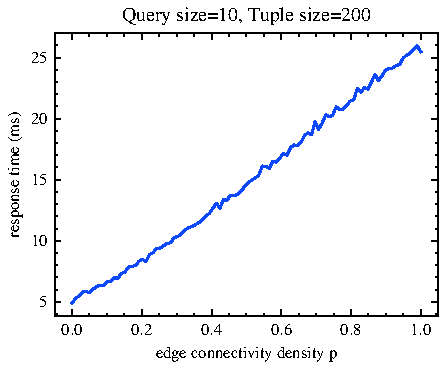
\includegraphics[width=0.6\textwidth]{my/graphics/tuple_completion_2.pdf}
	\caption{Optimal matching response time (ms) w.r.t. varying edge connectivity densities}
	\label{fig:tuple_completion_2}
\end{figure}
In our last step, we fix the query size and edge connectivity density to be the same as in step one, but change the tuple size so that it goes from 100 to 1,000. Again, we repeat the process for 100 times and compute the mean values. Figure~\ref{fig:tuple_completion_3} shows the results.
\begin{figure}[!th]
	\centering
	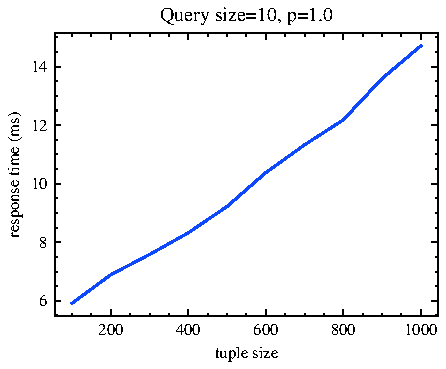
\includegraphics[width=0.6\textwidth]{my/graphics/tuple_completion_3.pdf}
	\caption{Optimal matching response time (ms) w.r.t. varying tuple sizes}
	\label{fig:tuple_completion_3}
\end{figure}

Our workloads A and B have query sizes of 3 and 5, respectively. The average number of attributes of the 10 datasets is less than 200. 
The experiment results from the above three steps indicate that the response time of optimal matching will be less than 30 milliseconds in our use case. 
The performance cost of optimal matching will not be as significant as that of full-text index lookup. 
Therefore, the majority of our work focuses on how to optimize index lookup using neural networks.

\subsection{Neural network based predictive access}
\label{subsection:nn_experiments}

We evaluate five neural network architectures including MLP, LSTM, Conv1D, Transformer and MLP-Mixer. While all of them can be made into deep networks, or in conjunction with other network architectures, our motivation is to make our models as small as possible so that they can be embedded in a search system.
Therefore, we focus on the minimalist approach to network design.

\subsubsection{Common experimental setup and evaluation metrics}
\noindent{\emph {Evaluation scenarios:}}
 We evaluate models with the following combination of different scenarios in all experiments:
\begin{itemize}
	\item We train the models using different sampling rates of attributes, as described in Section~\ref{subsection:training_data_gen}.
	\item We consider both word-based and 3-gram based training.
	\item We evaluate the performance of index scan using models' predictions
	and compare with the optimal and aggregate index lookup for each query in our query workloads.
\end{itemize}

\noindent{\emph {Tokenization and embedding of texts:}}
The tokens are either words or 3-grams of the values in the partial tuples.  Let $\mathbf{Voc}$ be the vocabulary.  The vocabulary size is determined by the attribute sampling rate during training. The vocabulary sizes are given in Table~\ref{tab:training_vocab_size}. Each token is embedded into $\mathbb{R}^{64}$ by a simple embedding layer that has
$|\mathbf{Voc}|\times 64$ parameters.

\noindent{\emph {Evaluation metrics:}}
We evaluate our models using the following metrics:
\begin{itemize}
\item Top-$k$ classification accuracy: since we know the true relations that contain the partial tuples in our query workloads, we can evaluate the classification accuracy of our model.  The top-$k$ accuracy is defined as the percentage of the correct label among the top-$k$ labels predicted.
\item Index lookup response time using the predicted access pattern: using the likelihoods produced by our model, we can sort the indexes by their likelihoods and access the most likely index first. The scan continues until the true relation is reached.
\end{itemize}

\subsubsection{Multilayer perceptron (MLP)}
\label{subsection:expt_mlp}

\noindent{\emph Description:}

Multilayer perceptron (MLP) is probably the most widely used neural network architecture.  In this experiment, we will test the effectiveness of MLP by itself with a single hidden layer.

\noindent{\emph {Model architecture:}}

\begin{itemize}
    \item Since each query is a sequence of tokens, each query is embedded into
    $\mathbb{R}^{L\times 64}$ where $L$ is the token sequence length.  We use global
    average pooling to generate a flat vector in $\mathbb{R}^{64}$, which is used as the input to the MLP layer.
    \item MLP has one hidden layer of size 100.
    \item We utilize one drop-out layer to prevent overfitting by the large embedding layer.
\end{itemize}

The overall network architecture can be found in Figure~\ref{fig:mlp_model}.
\begin{figure}[!th]
	\centering
	\includesvg[inkscapelatex=false, width = 250pt]{mlp_model.svg}
	\caption{MLP model}
	\label{fig:mlp_model}
\end{figure}
Since we have six sets of training datasets, we have 6 trained MLP models, as shown in Table \ref{tab:trained_mlp_models}.
\begin{table}[!th]
	\centering
	\begin{tabularx}{0.8\textwidth}{|l|X|}
		\hline
		\textbf{Model name} & \textbf{Training dataset} \\ \hline
		mlp100 & 100\% attrs., word-based \\
		mlp100-3gram\ & 100\% attrs., 3-gram based \\ 
		mlp75 & 75\% attrs., word-based \\
		mlp75-3gram & 75\% attrs., 3-gram based \\ 
		mlp50 & 50\% attrs., word-based \\
		mlp50-3gram & 50\% attrs., 3-gram based \\ 
		\hline
	\end{tabularx}
	\caption{MLP model names and corresponding training datasets.}
	\label{tab:trained_mlp_models}
\end{table}

\noindent{\emph Observations:}

\begin{itemize}
	\item The top-1 to top-5 accuracies for all variations of MLP models under the workloads A and B are shown in Figure~\ref{fig:top_k_mlp_all}. Word-based models perform better than 3-gram based models under both workloads, which do not contain misspelled and unknown keywords.
	\item Figure~\ref{fig:mlp_perf_all_A} and Figure~\ref{fig:mlp_perf_all_B} show the distribution of query processing time under the workloads A and B, respectively. Word-based models improve query processing more than 3-gram based models do. In addition, the models trained using partial tuples with less attributes perform better than those trained using partial tuples with more attributes.
\end{itemize}
\begin{figure}[!th]
	\centering
	\begin{subfigure}{0.45\textwidth}
		\centering
%		\includesvg[inkscapelatex=false]{top_k_mlp_A.svg}
		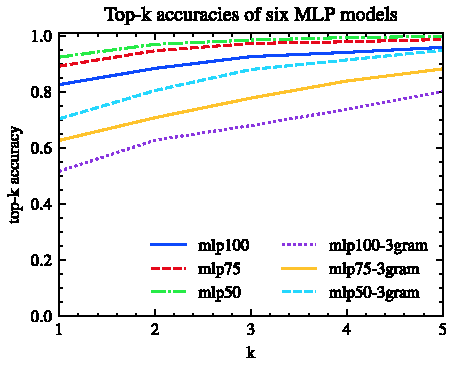
\includegraphics[]{my/graphics/top_k_mlp_A.pdf}
		\caption{Under the workload A.}
		\label{fig:top_k_mlp_A}
	\end{subfigure}
	\hfill
	\begin{subfigure}{0.45\textwidth}
		\centering
%		\includesvg[inkscapelatex=false]{top_k_mlp_B.svg}
		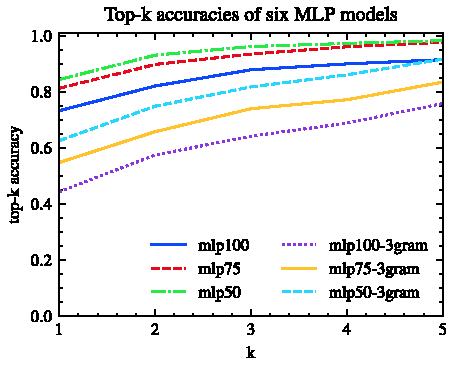
\includegraphics[]{my/graphics/top_k_mlp_B.pdf}
		\caption{Under the workload B.}
		\label{fig:top_k_mlp_B}
	\end{subfigure}
	\caption{Top-$k$ accuracies of six MLP models under the workload A and B.}
	\label{fig:top_k_mlp_all}
\end{figure}
\begin{figure}[!th]
	\centering
	\begin{subfigure}{0.45\textwidth}
		\begin{subfigure}{\textwidth}
			\centering
%			\includesvg[inkscapelatex=false]{perf_dist_mlp100_A.svg}
			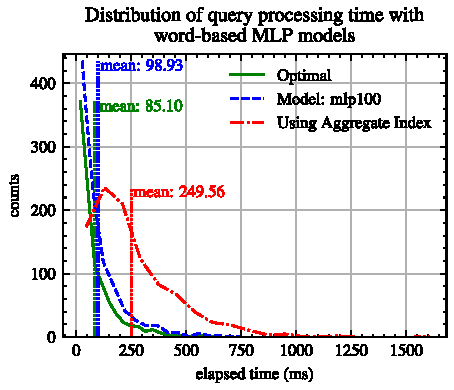
\includegraphics[]{my/graphics/perf_dist_mlp100_A.pdf}
		\end{subfigure}
		\vfill
		\begin{subfigure}{\textwidth}
			\centering
%			\includesvg[inkscapelatex=false]{perf_dist_mlp75_A.svg}
			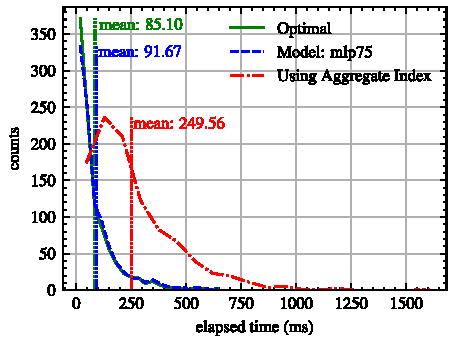
\includegraphics[]{my/graphics/perf_dist_mlp75_A.pdf}
		\end{subfigure}
		\vfill
		\begin{subfigure}{\textwidth}
			\centering
%			\includesvg[inkscapelatex=false]{perf_dist_mlp50_A.svg}
			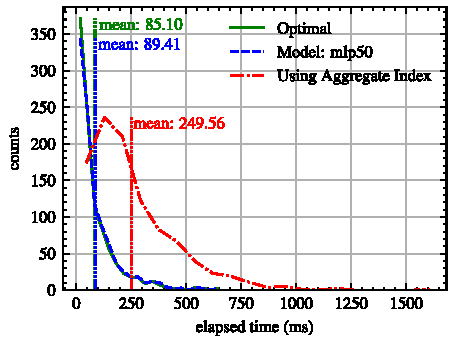
\includegraphics[]{my/graphics/perf_dist_mlp50_A.pdf}
		\end{subfigure}
		\caption{Word-based MLP models}
	\end{subfigure}
	\hfill
	\begin{subfigure}{0.45\textwidth}
		\begin{subfigure}{\textwidth}
			\centering
%			\includesvg[inkscapelatex=false]{perf_dist_mlp100_3gram_A.svg}
			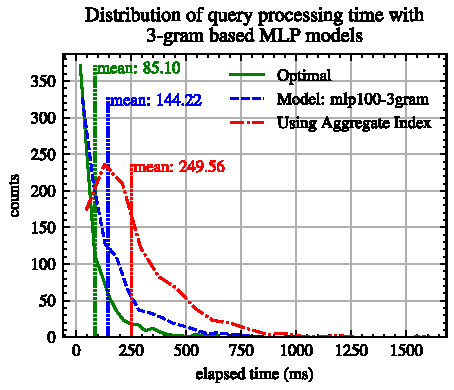
\includegraphics[]{my/graphics/perf_dist_mlp100_3gram_A.pdf}
		\end{subfigure}
		\vfill
		\begin{subfigure}{\textwidth}
			\centering
%			\includesvg[inkscapelatex=false]{perf_dist_mlp75_3gram_A.svg}
			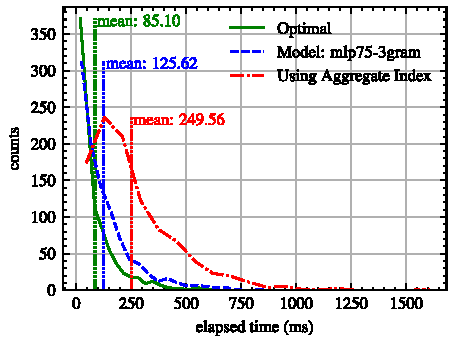
\includegraphics[]{my/graphics/perf_dist_mlp75_3gram_A.pdf}
		\end{subfigure}
		\vfill
		\begin{subfigure}{\textwidth}
			\centering
%			\includesvg[inkscapelatex=false]{perf_dist_mlp50_3gram_A.svg}
			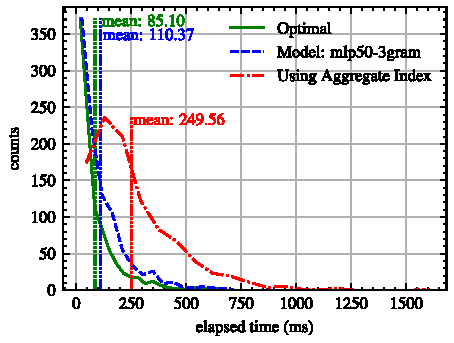
\includegraphics[]{my/graphics/perf_dist_mlp50_3gram_A.pdf}
		\end{subfigure}
		\caption{3-gram based MLP models}
	\end{subfigure}
	\caption{Distribution of query processing time with MLP models under the workload A.}
	\label{fig:mlp_perf_all_A}
\end{figure}
\begin{figure}[!th]
	\centering
	\begin{subfigure}{0.45\textwidth}
		\begin{subfigure}{\textwidth}
			\centering
%			\includesvg[inkscapelatex=false]{perf_dist_mlp100_B.svg}
			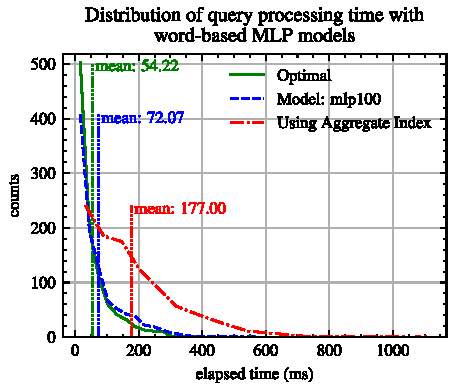
\includegraphics[]{my/graphics/perf_dist_mlp100_B.pdf}
		\end{subfigure}
		\vfill
		\begin{subfigure}{\textwidth}
			\centering
			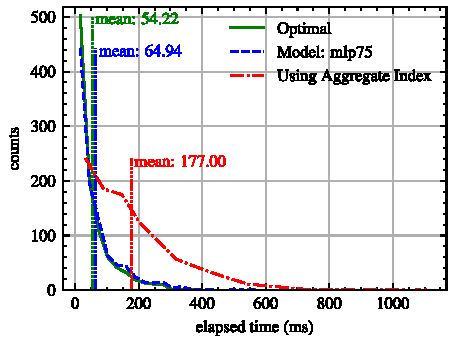
\includegraphics[]{my/graphics/perf_dist_mlp75_B.pdf}
		\end{subfigure}
		\vfill
		\begin{subfigure}{\textwidth}
			\centering
			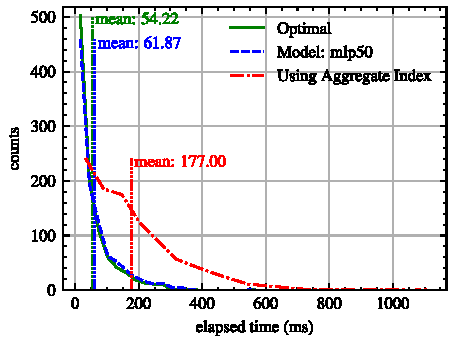
\includegraphics[]{my/graphics/perf_dist_mlp50_B.pdf}
		\end{subfigure}
		\caption{Word-based MLP models}
	\end{subfigure}
	\hfill
	\begin{subfigure}{0.45\textwidth}
		\begin{subfigure}{\textwidth}
			\centering
			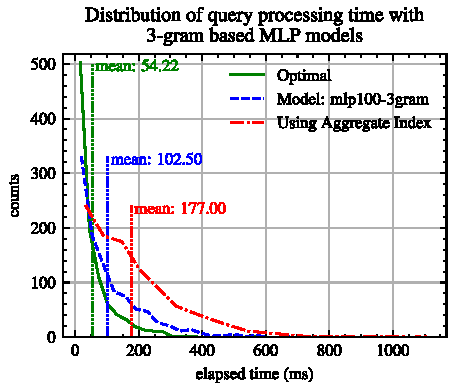
\includegraphics[]{my/graphics/perf_dist_mlp100_3gram_B.pdf}
		\end{subfigure}
		\vfill
		\begin{subfigure}{\textwidth}
			\centering
			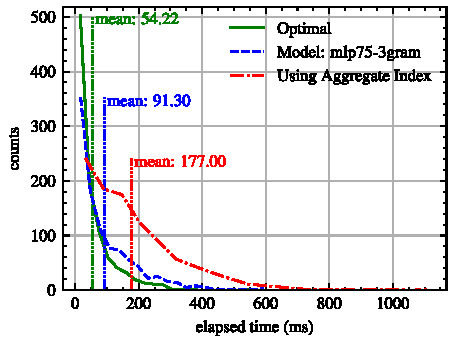
\includegraphics[]{my/graphics/perf_dist_mlp75_3gram_B.pdf}
		\end{subfigure}
		\vfill
		\begin{subfigure}{\textwidth}
			\centering
			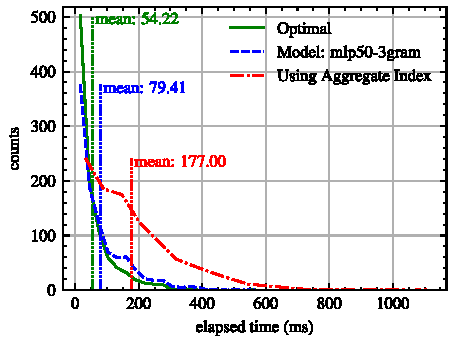
\includegraphics[]{my/graphics/perf_dist_mlp50_3gram_B.pdf}
		\end{subfigure}
		\caption{3-gram based MLP models}
	\end{subfigure}
	\caption{Distribution of query processing time with MLP models under the workload B.}
	\label{fig:mlp_perf_all_B}
\end{figure}

\subsubsection{Long short-term memory (LSTM)}

\noindent{\emph Description:}

Long short-term memory (LSTM) is a neural network architecture for sequence learning. Even though attributes in a tuple is not considered as a sequence since they are not ordered, the attribute values can be considered as short sequences of tokens. We test how LSTM performs when dealing with relational data in this experiment. Again we apply the minimalist approach to its network design by a single LSTM layer.

\noindent{\emph {Model architecture:}}

\begin{itemize}
	\item Each query is embedded into $\mathbb{R}^{L\times 64}$ where $L$ is the token sequence length, which is used as the input to the LSTM layer.
	\item We apply one drop-out layer to the output of the LSTM layer to prevent overfitting.
	\item The LSTM model has one hidden layer of size 100.
\end{itemize}

The model architecture is shown in Figure \ref{fig:lstm_model}. The 6 trained LSTM models are listed in Table~\ref{tab:trained_lstm_models}.
\begin{figure}[!th]
	\centering
	\includesvg[inkscapelatex=false, width = 250pt]{lstm_model.svg}
	\caption{LSTM model}
	\label{fig:lstm_model}
\end{figure}
\begin{table}[!th]
	\centering
	\begin{tabularx}{0.8\textwidth}{|l|X|}
		\hline
		\textbf{Model name} & \textbf{Training dataset} \\ \hline
		lstm100 & 100\% attrs., word-based \\
		lstm100-3gram & 100\% attrs., 3-gram based \\ 
		lstm75 & 75\% attrs., word-based \\
		lstm75-3gram & 75\% attrs., 3-gram based \\ 
		lstm50 & 50\% attrs., word-based \\
		lstm50-3gram & 50\% attrs., 3-gram based \\ 
		\hline
	\end{tabularx}
	\caption{LSTM model names and corresponding training datasets.}
	\label{tab:trained_lstm_models}
\end{table}

\noindent{\emph Observations:}

\begin{itemize}
	\item The top-1 to top-5 accuracies for all variations of LSTM models under the workloads A and B are shown in Figure~\ref{fig:top_k_lstm_all}. 
	Word-based models perform better than 3-gram based models. When compared to MLP models, LSTM models underperform under both workloads.
	\item Figure~\ref{fig:lstm_perf_all_A} and Figure~\ref{fig:lstm_perf_all_B} show the distribution of query processing time under the workloads A and B, respectively. 
	Word-based models improve query processing more than 3-gram based models do. 
	In addition, similar to MLP models, the models trained using partial tuples with less attributes perform better than those trained using partial tuples with more attributes.
\end{itemize}
\begin{figure}[!th]
	\centering
	\begin{subfigure}{0.45\textwidth}
		\centering
%		\includesvg[inkscapelatex=false]{top_k_lstm_A.svg}
		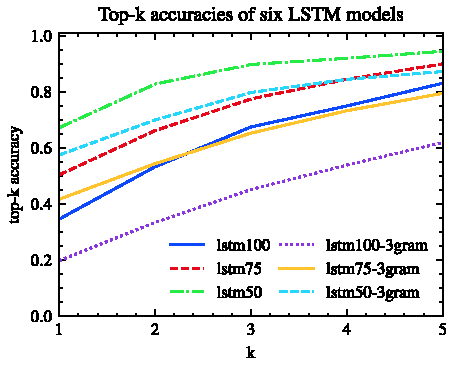
\includegraphics[]{my/graphics/top_k_lstm_A.pdf}
		\caption{Under the workload A.}
		\label{fig:top_k_lstm_A}
	\end{subfigure}
	\hfill
	\begin{subfigure}{0.45\textwidth}
		\centering
		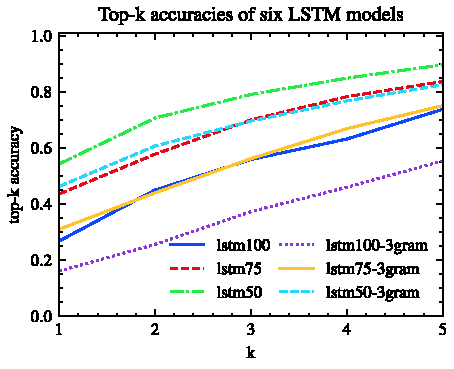
\includegraphics[]{my/graphics/top_k_lstm_B.pdf}
		\caption{Under the workload B.}
		\label{fig:top_k_lstm_B}
	\end{subfigure}
	\caption{Top-$k$ accuracies of six LSTM models under the workload A and B.}
	\label{fig:top_k_lstm_all}
\end{figure}
\begin{figure}[!th]
	\centering
	\begin{subfigure}{0.45\textwidth}
		\begin{subfigure}{\textwidth}
			\centering
%			\includesvg[inkscapelatex=false]{perf_dist_lstm100_A.svg}
			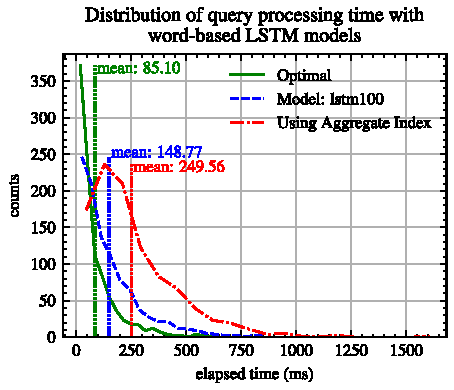
\includegraphics[]{my/graphics/perf_dist_lstm100_A.pdf}
		\end{subfigure}
		\vfill
		\begin{subfigure}{\textwidth}
			\centering
			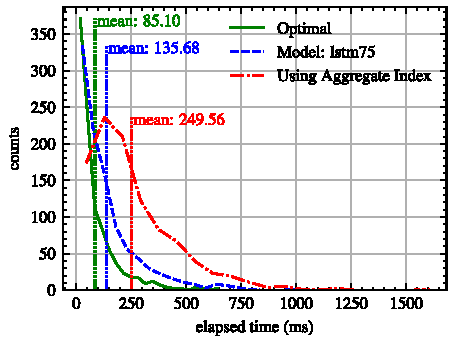
\includegraphics[]{my/graphics/perf_dist_lstm75_A.pdf}
		\end{subfigure}
		\vfill
		\begin{subfigure}{\textwidth}
			\centering
			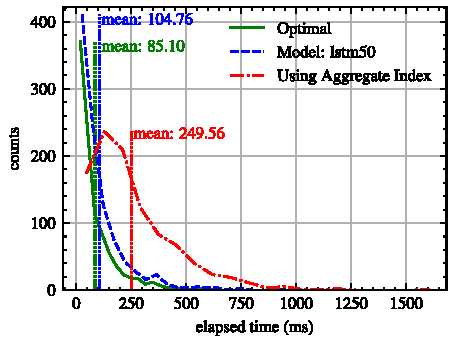
\includegraphics[]{my/graphics/perf_dist_lstm50_A.pdf}
		\end{subfigure}
		\caption{Word-based LSTM models}
	\end{subfigure}
	\hfill
	\begin{subfigure}{0.45\textwidth}
		\begin{subfigure}{\textwidth}
			\centering
			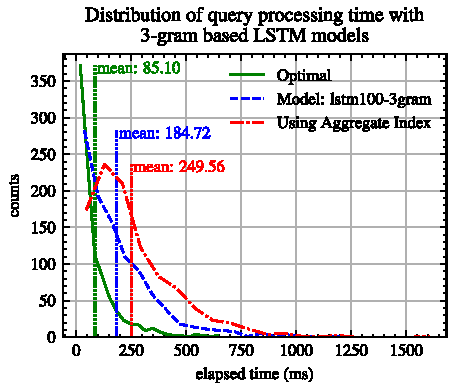
\includegraphics[]{my/graphics/perf_dist_lstm100_3gram_A.pdf}
		\end{subfigure}
		\vfill
		\begin{subfigure}{\textwidth}
			\centering
			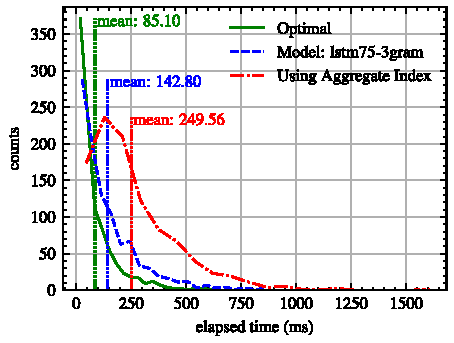
\includegraphics[]{my/graphics/perf_dist_lstm75_3gram_A.pdf}
		\end{subfigure}
		\vfill
		\begin{subfigure}{\textwidth}
			\centering
			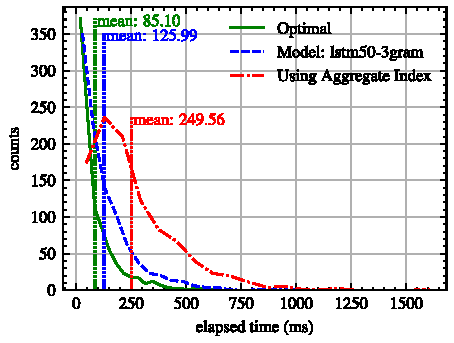
\includegraphics[]{my/graphics/perf_dist_lstm50_3gram_A.pdf}
		\end{subfigure}
		\caption{3-gram based LSTM models}
	\end{subfigure}
	\caption{Distribution of query processing time with LSTM models under the workload A.}
	\label{fig:lstm_perf_all_A}
\end{figure}
\begin{figure}[!th]
	\centering
	\begin{subfigure}{0.45\textwidth}
		\begin{subfigure}{\textwidth}
			\centering
%			\includesvg[inkscapelatex=false]{perf_dist_lstm100_B.svg}
			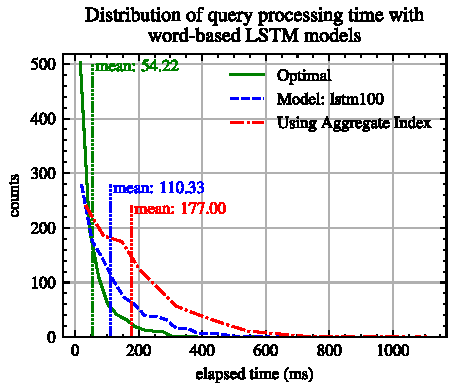
\includegraphics[]{my/graphics/perf_dist_lstm100_B.pdf}
		\end{subfigure}
		\vfill
		\begin{subfigure}{\textwidth}
			\centering
			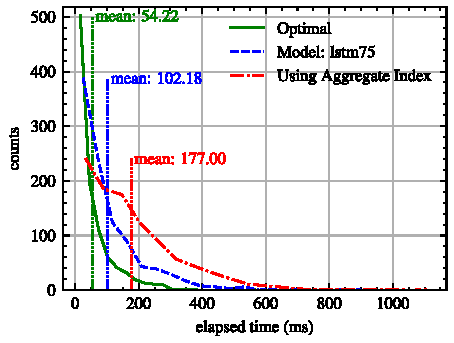
\includegraphics[]{my/graphics/perf_dist_lstm75_B.pdf}
		\end{subfigure}
		\vfill
		\begin{subfigure}{\textwidth}
			\centering
			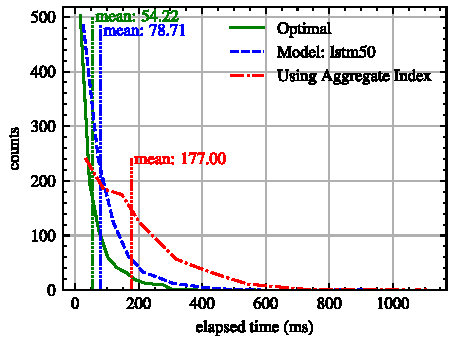
\includegraphics[]{my/graphics/perf_dist_lstm50_B.pdf}
		\end{subfigure}
		\caption{Word-based LSTM models}
	\end{subfigure}
	\hfill
	\begin{subfigure}{0.45\textwidth}
		\begin{subfigure}{\textwidth}
			\centering
			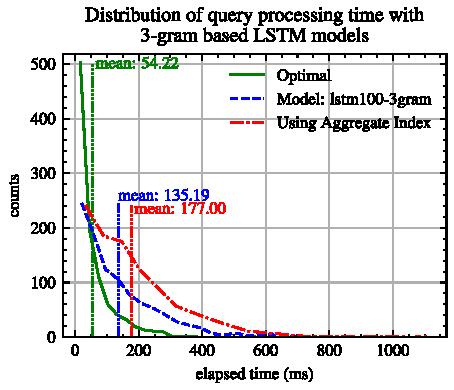
\includegraphics[]{my/graphics/perf_dist_lstm100_3gram_B.pdf}
		\end{subfigure}
		\vfill
		\begin{subfigure}{\textwidth}
			\centering
			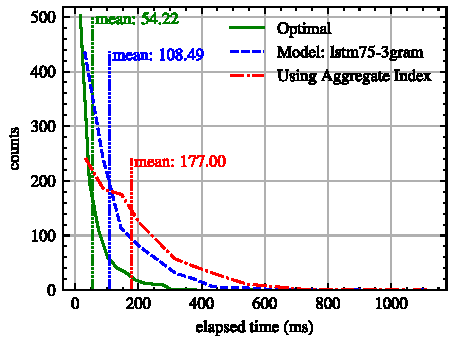
\includegraphics[]{my/graphics/perf_dist_lstm75_3gram_B.pdf}
		\end{subfigure}
		\vfill
		\begin{subfigure}{\textwidth}
			\centering
			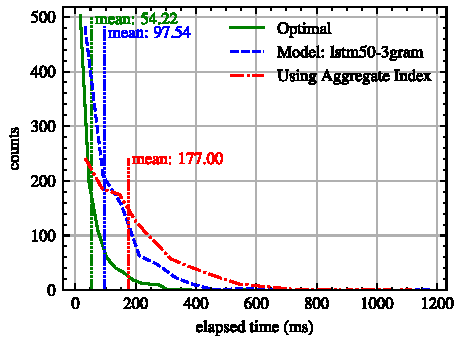
\includegraphics[]{my/graphics/perf_dist_lstm50_3gram_B.pdf}
		\end{subfigure}
		\caption{3-gram based LSTM models}
	\end{subfigure}
	\caption{Distribution of query processing time with LSTM models under the workload B.}
	\label{fig:lstm_perf_all_B}
\end{figure}

\subsubsection{One dimensional convolution (Conv1D)}

\noindent{\emph Description:}

Another way of doing sequence learning is 1-dimensional convolutional neural networks (Conv1D). Similar to what we do to LSTM, we want to see how Conv1D performs when processing relational data. We also minimize the network structure by using a single Conv1D layer.

\noindent{\emph {Model architecture:}}

\begin{itemize}
	\item Each query is embedded into $\mathbb{R}^{L\times 64}$ where $L$ is the token sequence length, which is used as the input to the Conv1D layer.
	\item The Conv1D layer has 64 kernels with kernel size of 3.
	\item We apply global average pooling to the output of Conv1D layer to generate a flat vector in $\mathbb{R}^{64}$.
	\item We apply one drop-out layer to the flattened vector to prevent overfitting.
\end{itemize}

The model architecture is shown in Figure~\ref{fig:conv1d_model}. The 6 trained Conv1D models are listed in Table~\ref{tab:trained_conv1d_models}.
\begin{figure}[!th]
	\centering
	\includesvg[inkscapelatex=false, width = 250pt]{conv1d_model.svg}
	\caption{Conv1D model}
	\label{fig:conv1d_model}
\end{figure}
\begin{table}[!th]
	\centering
	\begin{tabularx}{0.8\textwidth}{|l|X|}
		\hline
		\textbf{Model name} & \textbf{Training dataset} \\ \hline
		conv1d100 & 100\% attrs., word-based \\
		conv1d100-3gram & 100\% attrs., 3-gram based \\ 
		conv1d75 & 75\% attrs., word-based \\
		conv1d75-3gram & 75\% attrs., 3-gram based \\ 
		conv1d50 & 50\% attrs., word-based \\
		conv1d50-3gram & 50\% attrs., 3-gram based \\ 
		\hline
	\end{tabularx}
	\caption{Conv1D model names and corresponding training datasets.}
	\label{tab:trained_conv1d_models}
\end{table}

\noindent{\emph Observations:}

\begin{itemize}
	\item The top-1 to top-5 accuracies for all variations of Conv1D models under the workloads A and B are shown in Figure~\ref{fig:top_k_conv1d_all}. 
	Word-based models perform better than 3-gram based models.
	\item Figure~\ref{fig:conv1d_perf_all_A} and Figure~\ref{fig:conv1d_perf_all_B} show the distribution of query processing time under the workloads A and B, respectively. 
	Word-based models improve query processing more than 3-gram based models do. 
	Under the workload A, the 3-gram based models trained using partial tuples with less attributes perform better than those trained using partial tuples with more attributes, but the word-based models show an opposite relationship.
	Under the workload B, both word-based and 3-gram based models do better when trained using partial tuples with less attributes.
\end{itemize}
\begin{figure}[!th]
	\centering
	\begin{subfigure}{0.45\textwidth}
		\centering
		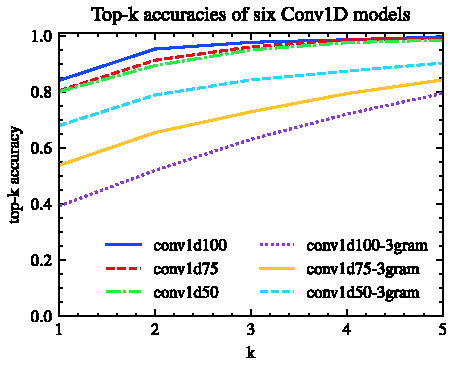
\includegraphics[]{my/graphics/top_k_conv1d_A.pdf}
		\caption{Under the workload A.}
		\label{fig:top_k_conv1d_A}
	\end{subfigure}
	\hfill
	\begin{subfigure}{0.45\textwidth}
		\centering
		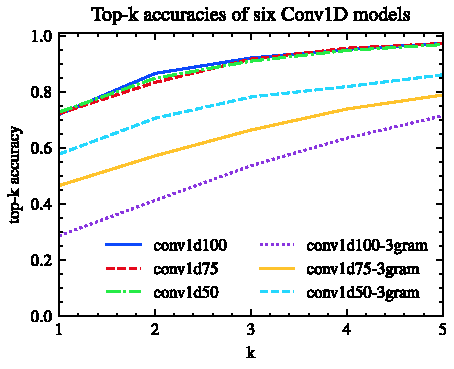
\includegraphics[]{my/graphics/top_k_conv1d_B.pdf}
		\caption{Under the workload B.}
		\label{fig:top_k_conv1d_B}
	\end{subfigure}
	\caption{Top-$k$ accuracies of six Conv1D models under the workload A and B.}
	\label{fig:top_k_conv1d_all}
\end{figure}
\begin{figure}[!h]
	\centering
	\begin{subfigure}{0.45\textwidth}
		\begin{subfigure}{\textwidth}
			\centering
			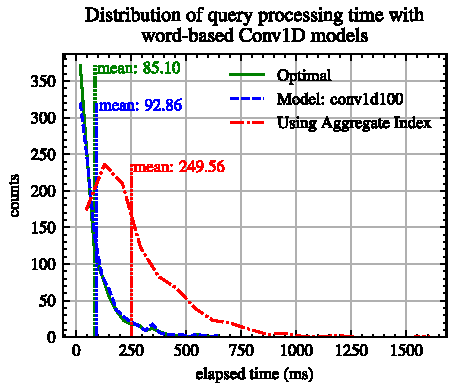
\includegraphics[]{my/graphics/perf_dist_conv1d100_A.pdf}
		\end{subfigure}
		\vfill
		\begin{subfigure}{\textwidth}
			\centering
			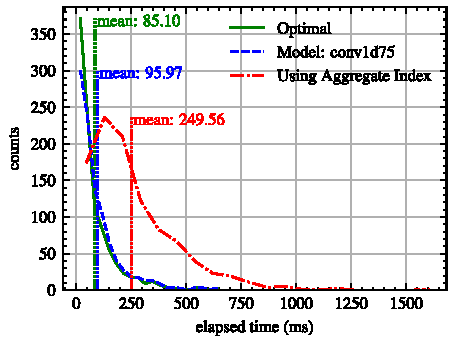
\includegraphics[]{my/graphics/perf_dist_conv1d75_A.pdf}
		\end{subfigure}
		\vfill
		\begin{subfigure}{\textwidth}
			\centering
			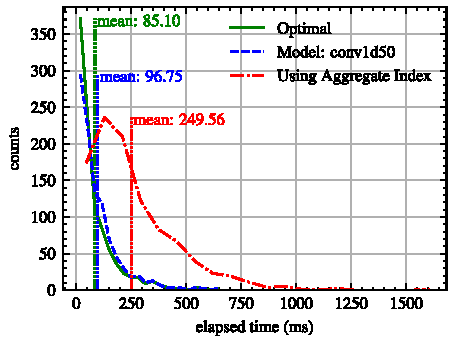
\includegraphics[]{my/graphics/perf_dist_conv1d50_A.pdf}
		\end{subfigure}
		\caption{Word-based Conv1D models}
	\end{subfigure}
	\hfill
	\begin{subfigure}{0.45\textwidth}
		\begin{subfigure}{\textwidth}
			\centering
			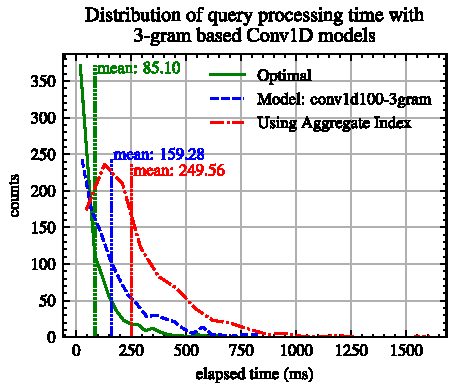
\includegraphics[]{my/graphics/perf_dist_conv1d100_3gram_A.pdf}
		\end{subfigure}
		\vfill
		\begin{subfigure}{\textwidth}
			\centering
			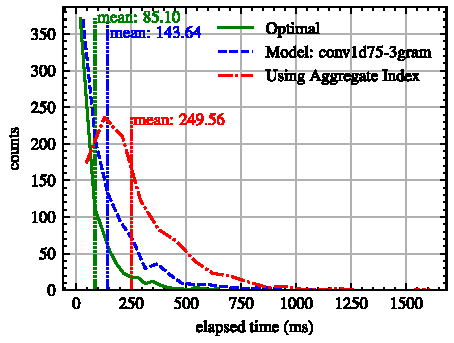
\includegraphics[]{my/graphics/perf_dist_conv1d75_3gram_A.pdf}
		\end{subfigure}
		\vfill
		\begin{subfigure}{\textwidth}
			\centering
			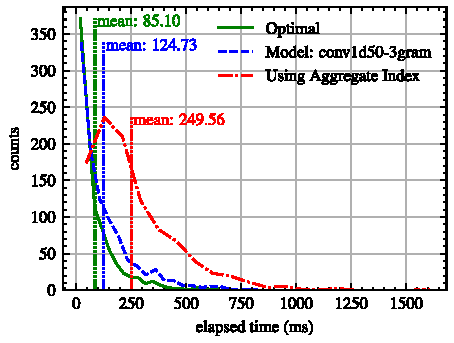
\includegraphics[]{my/graphics/perf_dist_conv1d50_3gram_A.pdf}
		\end{subfigure}
		\caption{3-gram based Conv1D models}
	\end{subfigure}
	\caption{Distribution of query processing time with Conv1D models under the workload A.}
	\label{fig:conv1d_perf_all_A}
\end{figure}
\begin{figure}[!h]
	\centering
	\begin{subfigure}{0.45\textwidth}
		\begin{subfigure}{\textwidth}
			\centering
			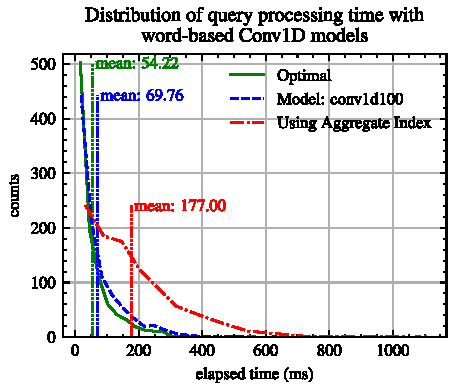
\includegraphics[]{my/graphics/perf_dist_conv1d100_B.pdf}
		\end{subfigure}
		\vfill
		\begin{subfigure}{\textwidth}
			\centering
			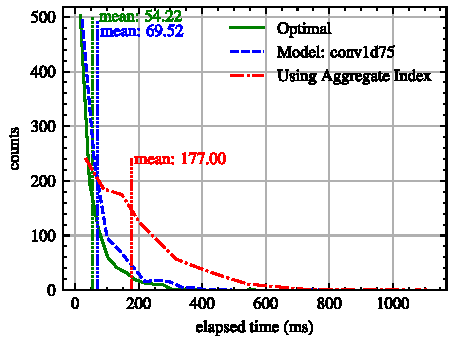
\includegraphics[]{my/graphics/perf_dist_conv1d75_B.pdf}
		\end{subfigure}
		\vfill
		\begin{subfigure}{\textwidth}
			\centering
			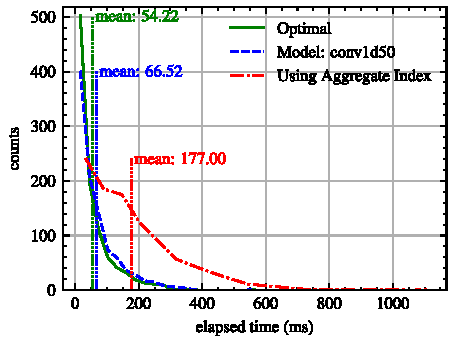
\includegraphics[]{my/graphics/perf_dist_conv1d50_B.pdf}
		\end{subfigure}
		\caption{Word-based Conv1D models}
	\end{subfigure}
	\hfill
	\begin{subfigure}{0.45\textwidth}
		\begin{subfigure}{\textwidth}
			\centering
			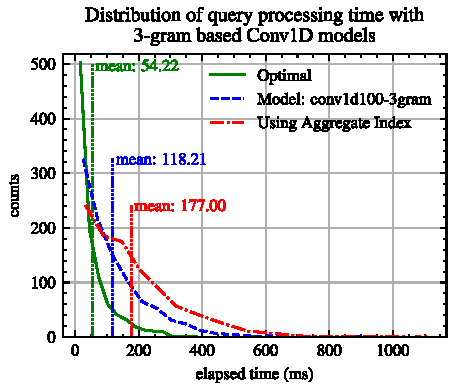
\includegraphics[]{my/graphics/perf_dist_conv1d100_3gram_B.pdf}
		\end{subfigure}
		\vfill
		\begin{subfigure}{\textwidth}
			\centering
			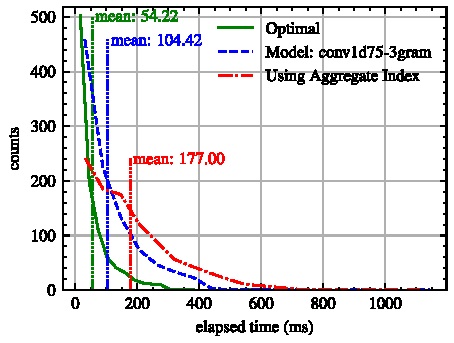
\includegraphics[]{my/graphics/perf_dist_conv1d75_3gram_B.pdf}
		\end{subfigure}
		\vfill
		\begin{subfigure}{\textwidth}
			\centering
			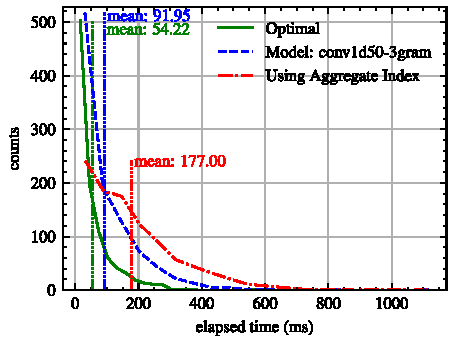
\includegraphics[]{my/graphics/perf_dist_conv1d50_3gram_B.pdf}
		\end{subfigure}
		\caption{3-gram based Conv1D models}
	\end{subfigure}
	\caption{Distribution of query processing time with Conv1D models under the workload B.}
	\label{fig:conv1d_perf_all_B}
\end{figure}

\subsubsection{Single transformer block}

\noindent{\emph Description:}

The Transformer architecture introduced in the original Transformer paper \cite{DBLP:journals/corr/VaswaniSPUJGKP17} is one of the main advances in natural language processing. In this experiment, we evaluate Transformer architecture for relational data. We largely follow the encoder architecture of the vanilla Transformer presented in the paper \cite{DBLP:journals/corr/VaswaniSPUJGKP17}. However, since our data are relational, we remove positional encoding. In addition, we only create one Transformer block to minimize the model architecture.

\noindent{\emph {Model architecture:}}

\begin{itemize}
	\item Each query is embedded into $\mathbb{R}^{L\times 64}$ where $L$ is the token sequence length, which is used as the input to the Transformer block.
	\item Inside the Transformer block, the attention layer has 4 attention heads. We add an extra drop-out layer after both the attention layer and the feed-forward network to prevent overfitting.
	\item The feed-forward network has a hidden layer of size 64.
	\item We apply global average pooling to the output of the Transformer block to generate a flat vector in $\mathbb{R}^{64}$.
        \item Then we apply a drop-out layer to the flattened vector.
\end{itemize}

Figure \ref{fig:transformer_model_all} shows its architecture. The 6 trained Transformer models are listed in Table~\ref{tab:trained_transformer_models}.
\begin{figure}[!th]
	\begin{subfigure}[]{0.4\textwidth}
		\begin{subfigure}[]{\textwidth}
			\centering
			\includesvg[inkscapelatex=false, width = \textwidth]{transformer_model.svg}
			\caption{Overall architecture}
			\label{fig:transformer_model}		
		\end{subfigure}
		\vfill
		\begin{subfigure}[]{\textwidth}
			\centering
			\includesvg[inkscapelatex=false, width = \textwidth]{transformer_model_ffn.svg}
			\caption{Feed-forward network}
			\label{fig:transformer_model_ffn}
		\end{subfigure}
	\end{subfigure}
	\hfill
	\centering
	\begin{subfigure}[]{0.5\textwidth}
		\centering
		\includesvg[inkscapelatex=false, width = \textwidth]{transformer_model_block.svg}
		\caption{Transformer block}
		\label{fig:transformer_model_block}
	\end{subfigure}
	\caption{Transformer model}
	\label{fig:transformer_model_all}
\end{figure}

\begin{table}[!th]
	\centering
	\begin{tabularx}{0.8\textwidth}{|l|X|}
		\hline
		\textbf{Model name} & \textbf{Training dataset} \\ \hline
		transformer100 & 100\% attrs., word-based \\
		transformer100-3gram & 100\% attrs., 3-gram based \\ 
		transformer75 & 75\% attrs., word-based \\
		transformer75-3gram & 75\% attrs., 3-gram based \\ 
		transformer50 & 50\% attrs., word-based \\
		transformer50-3gram & 50\% attrs., 3-gram based \\ 
		\hline
	\end{tabularx}
	\caption{Transformer model names and corresponding training datasets.}
	\label{tab:trained_transformer_models}
\end{table}
\noindent{\emph Observations:}

\begin{itemize}
	\item The top-1 to top-5 accuracies for all variations of Transformer models under the workloads A and B are shown in Figure~\ref{fig:top_k_transformer_all}. 
	Again, word-based models perform better than 3-gram based models. 
	\item Figure~\ref{fig:transformer_perf_all_A} and Figure~\ref{fig:transformer_perf_all_B} show the distribution of query processing time under the workloads A and B, respectively.
	Word-based models improve query processing more than 3-gram based models do.
	In addition, the models trained using partial tuples with less attributes perform better than those trained using partial tuples with more attributes.
\end{itemize}
\begin{figure}[!th]
	\centering
	\begin{subfigure}{0.45\textwidth}
		\centering
		\includegraphics[]{my/graphics/top_k_transformer_A.pdf}
		\caption{Under the workload A.}
		\label{fig:top_k_transformer_A}
	\end{subfigure}
	\hfill
	\begin{subfigure}{0.45\textwidth}
		\centering
		\includegraphics[]{my/graphics/top_k_transformer_B.pdf}
		\caption{Under the workload B.}
		\label{fig:top_k_transformer_B}
	\end{subfigure}
	\caption{Top-$k$ accuracies of six Transformer models under the workload A and B.}
	\label{fig:top_k_transformer_all}
\end{figure}
\begin{figure}[p]
	\centering
	\begin{subfigure}{0.45\textwidth}
		\begin{subfigure}{\textwidth}
			\centering
			\includegraphics[]{my/graphics/perf_dist_transformer100_A.pdf}
		\end{subfigure}
		\vfill
		\begin{subfigure}{\textwidth}
			\centering
			\includegraphics[]{my/graphics/perf_dist_transformer75_A.pdf}
		\end{subfigure}
		\vfill
		\begin{subfigure}{\textwidth}
			\centering
			\includegraphics[]{my/graphics/perf_dist_transformer50_A.pdf}
		\end{subfigure}
		\caption{Word-based Transformer models}
	\end{subfigure}
	\hfill
	\begin{subfigure}{0.45\textwidth}
		\begin{subfigure}{\textwidth}
			\centering
			\includegraphics[]{my/graphics/perf_dist_transformer100_3gram_A.pdf}
		\end{subfigure}
		\vfill
		\begin{subfigure}{\textwidth}
			\centering
			\includegraphics[]{my/graphics/perf_dist_transformer75_3gram_A.pdf}
		\end{subfigure}
		\vfill
		\begin{subfigure}{\textwidth}
			\centering
			\includegraphics[]{my/graphics/perf_dist_transformer50_3gram_A.pdf}
		\end{subfigure}
		\caption{3-gram based Transformer models}
	\end{subfigure}
	\caption{Distribution of query processing time with Transformer models under the workload A.}
	\label{fig:transformer_perf_all_A}
\end{figure}
\begin{figure}[p]
	\centering
	\begin{subfigure}{0.45\textwidth}
		\begin{subfigure}{\textwidth}
			\centering
			\includegraphics[]{my/graphics/perf_dist_transformer100_B.pdf}
		\end{subfigure}
		\vfill
		\begin{subfigure}{\textwidth}
			\centering
			\includegraphics[]{my/graphics/perf_dist_transformer75_B.pdf}
		\end{subfigure}
		\vfill
		\begin{subfigure}{\textwidth}
			\centering
			\includegraphics[]{my/graphics/perf_dist_transformer50_B.pdf}
		\end{subfigure}
		\caption{Word-based Transformer models}
	\end{subfigure}
	\hfill
	\begin{subfigure}{0.45\textwidth}
		\begin{subfigure}{\textwidth}
			\centering
			\includegraphics[]{my/graphics/perf_dist_transformer100_3gram_B.pdf}
		\end{subfigure}
		\vfill
		\begin{subfigure}{\textwidth}
			\centering
			\includegraphics[]{my/graphics/perf_dist_transformer75_3gram_B.pdf}
		\end{subfigure}
		\vfill
		\begin{subfigure}{\textwidth}
			\centering
			\includegraphics[]{my/graphics/perf_dist_transformer50_3gram_B.pdf}
		\end{subfigure}
		\caption{3-gram based Transformer models}
	\end{subfigure}
	\caption{Distribution of query processing time with Transformer models under the workload B.}
	\label{fig:transformer_perf_all_B}
\end{figure}

\subsubsection{MLP-Mixer}
\label{subsection:expt_mlpmixer}

\noindent{\emph Description:}

MLP-Mixer is an architecture based on MLPs only, which is proposed by Tolstikhin et al. \cite{DBLP:journals/corr/abs-2105-01601}. It is intended for computer vision. However, we want to see whether we could use it for our use case. In this experiment, we modify its architecture for text processing. The same minimalist approach and evaluation scenarios are used as in other experiments.

\noindent{\emph {Model architecture:}}

\begin{itemize}
	\item Each query is embedded into $\mathbb{R}^{L\times 64}$ where $L$ is the token sequence length, which is used as the input to the Mixer Layer.
	\item The Mixer Layer is implemented following the architecture presented in the paper \cite{DBLP:journals/corr/abs-2105-01601}.
	\item Layer normalization is applied to outputs from the Mixer Layer.
	\item We apply global max pooling to the outputs of layer normalization to generate a flat vector in $\mathbb{R}^{64}$, which is used as input to the output layer.
\end{itemize}
Figure \ref{fig:mlpmixer_model_all} shows its architecture. The 6 trained MLP-Mixer models are listed in Table~\ref{tab:trained_mlpmixer_models}.
\begin{figure}[p]
	\centering
	\begin{subfigure}{\textwidth}
		\begin{subfigure}[t]{0.45\textwidth}
			\centering
			\includesvg[inkscapelatex=false, width=\textwidth]{mlpmixer_model_token_mixing.svg}
			\caption{Token mixing}
			\label{fig:mlpmixer_model_token_mixing}
		\end{subfigure}
		\hfill
		\begin{subfigure}[t]{0.45\textwidth}
			\centering
			\includesvg[inkscapelatex=false, width=\textwidth]{mlpmixer_model_channel_mixing.svg}
			\caption{Channel mixing}
			\label{fig:mlpmixer_model_channel_mixing}
		\end{subfigure}
	\end{subfigure}
	\vfill
	\begin{subfigure}{\textwidth}
		\begin{subfigure}[b]{0.4\textwidth}
			\centering
			\includesvg[inkscapelatex=false, width=\textwidth]{mlpmixer_model_mixer.svg}
			\caption{Mixer Layer}
			\label{fig:mlpmixer_model_mixer}
		\end{subfigure}
		\hfill
		\begin{subfigure}[b]{0.4\textwidth}
			\centering
			\includesvg[inkscapelatex=false, width=\textwidth]{mlpmixer_model.svg}
			\caption{Overall architecture}
			\label{fig:mlpmixer_model}
		\end{subfigure}
	\end{subfigure}
	\caption{MLP-Mixer model}
	\label{fig:mlpmixer_model_all}
\end{figure}
\begin{table}[!th]
	\centering
	\begin{tabularx}{0.8\textwidth}{|l|X|}
		\hline
		\textbf{Model name} & \textbf{Training dataset} \\ \hline
		mlpmixer100 & 100\% attrs., word-based \\
		mlpmixer100-3gram & 100\% attrs., 3-gram based \\ 
		mlpmixer75 & 75\% attrs., word-based \\
		mlpmixer75-3gram & 75\% attrs., 3-gram based \\ 
		mlpmixer50 & 50\% attrs., word-based \\
		mlpmixer50-3gram & 50\% attrs., 3-gram based \\ 
		\hline
	\end{tabularx}
	\caption{MLP-Mixer model names and corresponding training datasets.}
	\label{tab:trained_mlpmixer_models}
\end{table}

\noindent{\emph Observations:}

\begin{itemize}
	\item The top-1 to top-5 accuracies for all variations of MLP-Mixer models under the workloads A and B are shown in Figure~\ref{fig:top_k_mlpmixer_all}.
	\item Figure~\ref{fig:mlpmixer_perf_all_A} and Figure~\ref{fig:mlpmixer_perf_all_B} show the distribution of query processing time under the workloads A and B, respectively.
	The word-based models perform slightly better than 3-gram based models, with the exception of two models $\emph mlpmixer75$ and $\emph mlpmixer75$-$3gram$.
	In addition, the models trained using partial tuples with less attributes perform better than those trained using partial tuples with more attributes, 
	with the exception of the model $\emph mlpmixer75$ under the workload B.
\end{itemize}
\begin{figure}[!th]
	\centering
	\begin{subfigure}{0.45\textwidth}
		\centering
		\includegraphics[]{my/graphics/top_k_mlpmixer_A.pdf}
		\caption{Under the workload A.}
		\label{fig:top_k_mlpmixer_A}
	\end{subfigure}
	\hfill
	\begin{subfigure}{0.45\textwidth}
		\centering
		\includegraphics[]{my/graphics/top_k_mlpmixer_B.pdf}
		\caption{Under the workload B.}
		\label{fig:top_k_mlpmixer_B}
	\end{subfigure}
	\caption{Top-$k$ accuracies of six MLP-Mixer models under the workload A and B.}
	\label{fig:top_k_mlpmixer_all}
\end{figure}
\begin{figure}[!h]
	\centering
	\begin{subfigure}{0.45\textwidth}
		\begin{subfigure}{\textwidth}
			\centering
			\includegraphics[]{my/graphics/perf_dist_mlpmixer100_A.pdf}
		\end{subfigure}
		\vfill
		\begin{subfigure}{\textwidth}
			\centering
			\includegraphics[]{my/graphics/perf_dist_mlpmixer75_A.pdf}
		\end{subfigure}
		\vfill
		\begin{subfigure}{\textwidth}
			\centering
			\includegraphics[]{my/graphics/perf_dist_mlpmixer50_A.pdf}
		\end{subfigure}
		\caption{Word-based MLP-Mixer models}
	\end{subfigure}
	\hfill
	\begin{subfigure}{0.45\textwidth}
		\begin{subfigure}{\textwidth}
			\centering
			\includegraphics[]{my/graphics/perf_dist_mlpmixer100_3gram_A.pdf}
		\end{subfigure}
		\vfill
		\begin{subfigure}{\textwidth}
			\centering
			\includegraphics[]{my/graphics/perf_dist_mlpmixer75_3gram_A.pdf}
		\end{subfigure}
		\vfill
		\begin{subfigure}{\textwidth}
			\centering
			\includegraphics[]{my/graphics/perf_dist_mlpmixer50_3gram_A.pdf}
		\end{subfigure}
		\caption{3-gram based MLP-Mixer models}
	\end{subfigure}
	\caption{Distribution of query processing time with MLP-Mixer models under the workload A.}
	\label{fig:mlpmixer_perf_all_A}
\end{figure}
\begin{figure}[!h]
	\centering
	\begin{subfigure}{0.45\textwidth}
		\begin{subfigure}{\textwidth}
			\centering
			\includegraphics[]{my/graphics/perf_dist_mlpmixer100_B.pdf}
		\end{subfigure}
		\vfill
		\begin{subfigure}{\textwidth}
			\centering
			\includegraphics[]{my/graphics/perf_dist_mlpmixer75_B.pdf}
		\end{subfigure}
		\vfill
		\begin{subfigure}{\textwidth}
			\centering
			\includegraphics[]{my/graphics/perf_dist_mlpmixer50_B.pdf}
		\end{subfigure}
		\caption{Word-based MLP-Mixer models}
	\end{subfigure}
	\hfill
	\begin{subfigure}{0.45\textwidth}
		\begin{subfigure}{\textwidth}
			\centering
			\includegraphics[]{my/graphics/perf_dist_mlpmixer100_3gram_B.pdf}
		\end{subfigure}
		\vfill
		\begin{subfigure}{\textwidth}
			\centering
			\includegraphics[]{my/graphics/perf_dist_mlpmixer75_3gram_B.pdf}
		\end{subfigure}
		\vfill
		\begin{subfigure}{\textwidth}
			\centering
			\includegraphics[]{my/graphics/perf_dist_mlpmixer50_3gram_B.pdf}
		\end{subfigure}
		\caption{3-gram based MLP-Mixer models}
	\end{subfigure}
	\caption{Distribution of query processing time with MLP-Mixer models under the workload B.}
	\label{fig:mlpmixer_perf_all_B}
\end{figure}

\subsubsection{Comparison of different models}

Based on the observations from Section~\ref{subsection:expt_mlp} to Section~\ref{subsection:expt_mlpmixer}, we have compiled the following table to compare their relative performances with respect to the optimal and the aggregate index lookup under the workload A.

\begin{table}[ht]
    \centering
    \begin{tabularx}{\textwidth}{|l|X||X|X||X|X|X|}
    \hline
    &    \multicolumn{3}{|c|}{Word tokens} & \multicolumn{3}{|c|}{3-gram tokens} \\ \hline
    Model 
        & parameters
        & $\frac{\mathrm{model}}{\mathrm{optimal}}$
        & $\frac{\mathrm{model}}{\mathrm{aggr}}$ 
        & parameters
        & $\frac{\mathrm{model}}{\mathrm{optimal}}$
        & $\frac{\mathrm{model}}{\mathrm{aggr}}$
        \\ \hline
    MLP & 3.02M & {\bf 1.10} & 0.37 & 272K & {\bf 1.49} & 0.51\\
    LSTM & 3.05M & 1.52 & 0.52 & 305K & 1.78 & 0.61 \\
    Conv1D & 3.03M & {\bf 1.12} & 0.38 & 277K & 1.68 & 0.57 \\
    Transformer & 3.09M & {\bf 1.12} & 0.38 & 340K & {\bf 1.66} & 0.57 \\
    MLP Mixer & 3.04M & 1.65 & 0.56 & 287K & {\bf 1.65} & 0.56 \\ \hline
    \end{tabularx}
    \caption{Comparison of models under the workload A with the top-3 measurements highlighted.}
    \label{tab:model-comparison}
\end{table}

The observation supports our proposal of utilizing neural networks to accelerate
index lookup.  As shown in Table~\ref{tab:model-comparison}, many of the models perform well compared to the optimal index lookup, and significantly outperform the aggregate index lookup.

For word based tokens, MLP is only 10\% slower than the optimal index lookup, and outperforms the aggregate index by almost 3 times. The Conv1D and Transformer are only slightly worse than MLP. But the transformer models have larger model sizes. Both LSTM and MLP Mixer do not perform that well when compared to the other three networks.

We realize that we only use one transformer block and one MLP Mixer Layer, respectively.  In our context, we are interested in embedded networks as part of the query processor. Therefore, our focus is limited to small network architectures.

Regarding the model sizes, the main source of parameters is the embedding layer.
Word based tokens produce far more bigger vocabulary, which then requires many more
embedding vectors as model parameters.  The vocabulary of 3-grams is much smaller, and thus produces much more compact models.

Since 3-gram tokens individually capture less information than word-based tokens, we expect the observed performance degradation when using the 3-gram tokens. With that being said, MLP has shown to outperform the aggregate index with twice the performance even for 3-grams.

The value of 3-gram vocabularies becomes more apparent in scenarios with noisy queries.  When query strings contain spelling and other noises at a sub-word level, the two methods of tokenization, i.e., word-based and 3-gram based, behave quite differently.
For word-based tokenization, noisy words will generate out-of-vocabulary (OOV) tokens
which do not contribute to the classification of the network.  However, the 3-gram tokenization can still produce {\em some} 3-gram tokens even for misspelled and unknown words in a query string.  The next section is dedicated to evaluate how well word-based and 3-gram based networks behave in the presence of noisy queries.

\subsection{Impact of noisy queries on models' performance}
\label{subsection:expt_3gram_resiliency}

\noindent{\emph Descriptions:}

In this experiment, we investigate the impact of misspelled words in queries on the models' performance of top-5 accuracy. We simulate the scenario by replacing a randomly selected character in a word with the special character ``\_". For example, the city name \verb|toronto| becomes \verb|to_onto| after mutation. Its 3-gram tokens will be \verb|[__t, _to, to_, o_o, _on, ont, nto, to_, o__]|.

\noindent{\emph {Observations:}}

The impact of noisy queries on models' performance of top-5 accuracy is shown in Figure \ref{fig:acc_degradation_workload_A_all} and \ref{fig:acc_degradation_workload_B_all}  under  the workload A and B, respectively. The performance degradation of word-based models is much faster than that of 3-gram based models. This clearly shows that 3-gram based models are more resilient to query noises.
\begin{figure}[!th]
	\centering
	\begin{subfigure}[t]{0.95\textwidth}
		\includegraphics[]{my/graphics/acc_degradation_word_based_A.pdf}
		\caption{Word-based models}
		\label{fig:acc_degradation_workload_A_word_based}
	\end{subfigure}
	\vfill
	\begin{subfigure}[t]{0.95\textwidth}
		\includegraphics[]{my/graphics/acc_degradation_3gram_based_A.pdf}
		\caption{3-gram based models}
		\label{fig:acc_degradation_workload_A_3gram}
	\end{subfigure}
	\caption{Top-5 accuracy degradation of all models under the workload A.}
	\label{fig:acc_degradation_workload_A_all}
\end{figure}
\begin{figure}[!th]
	\centering
	\begin{subfigure}[]{0.95\textwidth}
		\includegraphics[]{my/graphics/acc_degradation_word_based_B.pdf}
		\caption{Word-based models}
		\label{fig:acc_degradation_workload_B_word_based}
	\end{subfigure}
	\vfill
	\begin{subfigure}[]{0.95\textwidth}
		\includegraphics[]{my/graphics/acc_degradation_3gram_based_B.pdf}
		\caption{3-gram based models}
		\label{fig:acc_degradation_workload_B_3gram}
	\end{subfigure}
	\caption{Top-5 accuracy degradation of all models under the workload B3.}
	\label{fig:acc_degradation_workload_B_all}
\end{figure}


\chapter{Related Work}

\section{Relational keyword search}
A lot of work has been done for relational keyword search. In this section, we review some of the previous works.

\noindent{\bf{Early papers:}} Hristidis and Papakonstantinou \cite{hristidis2002discover} presented DISCOVER, a system that allowed users to submit keyword queries to relational databases without the knowledge of the underlying database schema. DISCOVER processes keyword queries to generate candidate networks of relations and create execution plans to be submitted to RDBMS, which will return search results.
Liu et al. \cite{liu2006effective} proposed an information retrieval (IR) ranking strategy for effective keyword search related to relational databases. The ranking strategy used four normalization factors for computing ranking scores. 
All answers of a query were ranked based on computed ranking scores, and the top-$k$ answers were returned as results.

\noindent{\bf{Extension to include frequent co-occurring term (FCT):}} Tao and Yu \cite{tao2009finding} proposed an operator called frequent co-occurring term (FCT) search, and an algorithm that could solve FCT search effectively without using the conventional keyword search methods. The purpose of FCT search is to extract the terms that most accurately represent a set of keywords, i.e., to discover the concepts closely related to the keywords set.

\noindent{\bf{Survey of keyword search:}} A survey about research on keyword search in relational databases was done by Park and Lee \cite{park2011keyword}. First they listed fundamental characteristics of keyword search in relational databases: an indexing structure, being able to formalize internal queries based on query keywords, being able to correctly constructing candidate answers, and an answer ranking strategy. Then they investigated five research dimensions, including data representation, ranking, efficient processing, query representation, and result presentation. At the end, they pointed out some promising research directions. One of them is efficient top-$k$ query processing. The authors believed that keyword search in relational databases would benefit from advance in top-$k$ query processing techniques.


\noindent{\bf{Interpretation of keywords in query:}} Zeng et al. \cite{zeng2012isearch} presented a framework based on keyword query interpretations. It incorporated human feedback to remove keyword vaguenesses and use a ranking model for query interpretation evaluation afterwards.

\noindent{\bf{Top-$k$ recommendation:}} Meng et al. \cite{meng2017top} presented an approach to solve typical and semantically related queries to a given query. This can help users to explore their query intentions and improve their query formulation.



\section{Machine learning based database optimization}

\noindent{\bf{Index optimization:}} Ding et al. \cite{ding2020alex} presented an updatable learned index called ALEX, an in-memory index structure, for index optimization. ALEX addressed practical issues related to various types of workloads with dynamic updates. RadixSpline \cite{kipf2020radixspline}, another learned index, tackled the issue of index implementation difficulty. RadixSpline offered quick build using a single pass over data while achieving competitive performance.

\noindent{\bf{Query optimization:}} Bao \cite{marcus2022bao} is a learned query optimization system using reinforcement learning. It can learn from mistakes and adapt to dynamic workloads, data, and schema, thus is capable of applying per-query optimization hints.

\noindent{\bf{Cost models for query processing:}} Siddiqui1 et al. \cite{siddiqui2020cost} investigated how to learn cost models from cloud workloads for big data systems. The learned cost models could be integrated with existing query optimizers. Such a query optimizer could make accurate cost predictions, which can improve resource efficiency in big data systems.

\chapter{Conclusions and Future Work}
In this chapter, we summarize our work and describe possible continuing work that could be done in future.

\section{Summary}
Contributions from our work can be summarized as:
\begin{itemize}
    \item We propose partial tuple search as an extension of keyword search over relational data. It is a generalization of keyword search by allowing users to submit partial tuple queries, which can have both value-based keywords and schema-based structure information. Partial tuple search can be used by users with limited, but nonzero, knowledge over the schema of the underlying relational database.
    
    \item We demonstrate a query processing pipeline that can evaluate partial tuple search queries efficiently. 
    It consists of four main steps: convert a partial tuple to a keyword query,
    use an embedded neural network classifier to predict a dynamic access pattern of partitioned full-text indexes based on the keyword query, scan indexes to find top-$k$ candidates, and finally complete the partial tuple by finding an optimal match.
    
    The pipeline requires indexing each relation to a separate full-text index. It also needs a trained neural network classifier using sampled tuples from each relation.
    
    \item We identify bottleneck related to performing fuzzy string matching when using a monolithic full-text index. The bottleneck is related to the inverted index data structure used in a full-text index. When using $3$-gram tokenization to support fuzzy string matching, severe hash collision will happen because the number of documents is a lot bigger than that of 3-gram search terms. The performance will degrade from log-time $\mathcal{O}(\log n)$ to sequential scan $\mathcal{O}(n)$.

    \item We design an index partition scheme to speed up index lookup. We partition tuples by their corresponding relations, i.e., each relation is indexed into a separate full-text index. The partitioned indexes give us an opportunity to optimize query evaluation by using a neural network. This approach does not incur the additional costs of parallel CPU loads.
    
    \item We design self-supervised neural networks to optimize partitioned index access, which is incorporated in the query processing pipeline. We use relation names as labels to avoid manual labelling of training data, which are generated using sampled tuples from each relation. 
    
    \item Our experimental evaluation shows that small neural networks work well for our use case. Our MLP models perform particularly well, while Conv1D models and MLP based transformer models are pretty close. On the other hand, the 3-grams trained networks are highly robust w.r.t. spelling errors.
    
\end{itemize}


\section{Discussion of limitations and Future work}
\label{sec:limitation}
As described in Section~\ref{sec:assumption}, we assume that the counts of relations' tuples are not skewed, and that the vocabulary of the database is not affected by any operation applied to the database. 

If the first assumption is violated, for example, one relation has an extremely large number of tuples, our approach of partitioning index based on relations can not effectively tackle the bottleneck related to the inverted index any more. The partitioned indexes corresponding to large relations will have the same bottleneck caused by hashing collision in the inverted index data structure. Therefore, we will have to partition large relations based on some criteria. The key is to have the resultant partitions having different vocabularies, which could help training a more accurate neural network. We could partition a large relation by attributes or attribute values.
\begin{itemize}
    \item Partition a large relation by dividing its attributes into subsets. An intuition is to group attributes with similar vocabulary into the same partition. Thus, different partitions are likely to have quite different vocabularies. 
    \item Partition a large relation based on certain attribute values. For example, if a relation has an attribute about ``city'', we can divide the relation by city names. Each partition holds the data for a continuous range of the first letter of the city name, e.g., A-I, J-R and S-Z. The key of this approach is to pick an appropriate partition key for the relation.
    \item To the end of having partitions with vocabularies as different as possible, the first partitioning scheme could be a better option. This is because different attributes in a relation usually have different sets of limited values. On the other hand, partitions resulting from grouping by certain attribute values will have the same schema as the original relation, which means they are more likely to have similar vocabulary.
\end{itemize}
This is a possible future work direction that can improve the solutions proposed in the thesis.

Regarding the second assumption, if the vocabulary of the database changes, we can apply fine-tuning to the neural network classifier.
\begin{itemize}
    \item We freeze the network and apply incremental fine-tuning to embeddings only. We could freeze existing embeddings and only train new embeddings, or fine-tune all embeddings.
    \item We don't freeze the network. We simply apply fine-tuning to both embeddings and the network. This approach will take longer training time than the first approach. But since our network is relatively small, the extra training time is likely not significant.
\end{itemize}
This can be another direction of future work.

The current sizes of our neural networks are small enough to be embedded in a mobile application. For deployment scenarios involving a backend server, we can relax its size limit. This means that we can design deeper neural network architectures that are still embeddable in a system running on a server. In order to do that, we will need to resort to automatic tuning of hyperparameters to find optimal network designs. This can be an interesting future work, too.

Our work uses full-text index, Apache Lucene in particular, to index relational data and evaluate partial tuple queries. A possible future work is to integrate partial tuple search into existing RDBMS. This would give users a more flexible and powerful way to query relational databases.


\backmatter
\printbibliography[heading=bibintoc]
\end{document}
